\documentclass{article}
\usepackage[utf8]{inputenc}
\usepackage{rotating} % Creates an environment for a rotated figure.
\usepackage[letterpaper, margin=1in]{geometry}

\usepackage[printwatermark]{xwatermark} % Adds ability to use a watermark.
\usepackage{xcolor}
\usepackage{graphicx,wrapfig} % Adds graphics tools.
\newwatermark[allpages,color=red!50,angle=45,scale=3,xpos=0,ypos=0]{DRAFT}

\usepackage[english]{babel} % Allows me to change built-in macros. For this, I'm renaming "Figures" to "Attachments".
\addto\captionsenglish{%
  \renewcommand\listfigurename{List of Attachments}%
  \renewcommand\figurename{Attachment}%
  \renewcommand\contentsname{List of Contents}}
% \renewcommand{\figurename}{Attachment}
% \renewcommand{\listfigurename}{Attachments}

\usepackage{csquotes} % Allows the usage of \displayquote for block quotes.

\usepackage{natbib,hyperref} % Basic bibliography stuff.
\bibliographystyle{apalike}

% \usepackage{tikz}
% \usetikzlibrary{shapes.geometric, arrows}

\usepackage{soul} % Adds the \ul{} command so that underlining can break across lines.
\usepackage{color} % Adds color to text.
\DeclareRobustCommand{\hlcyan}[1]{{\sethlcolor{cyan}\hl{#1}}} % Defines the command \hlcyan{} to highlight in blue.
\DeclareRobustCommand{\hlbrown}[1]{{\sethlcolor{brown}\hl{#1}}} % Defines the command \hlcyan{} to highlight in blue.

\usepackage{todonotes} % Allows visible commenting.

\usepackage{graphicx} % Allows me to insert images into the document.
\graphicspath{ {images/} }
\usepackage{imakeidx} % Indexing package for the document.
\makeindex

\usepackage[toc,page]{appendix} % Allows me to separate an appendix section for additional documents.
\usepackage[final]{pdfpages} % Allows me to attach PDFs in the exported document.
\usepackage{pdflscape} % Allows PDFs to be rotated.

\title{Ipas Legal Storehouse -- Field work log}
\author{Tim D'Annecy}
\date{Summer 2016}

\begin{document}

\maketitle

\clearpage
\tableofcontents
\listoffigures
\clearpage

\section{Introduction}
The plan for the Field Experience is relatively straightforward, but it has taken a while to get off the ground and a lot has changed since its inception. This document will be a log of my work and will hopefully serve as a reference point for future work on this project. I'll also try to include notes about technical steps so that others can understand what I did.

\section{January 25, 2016}
\subsection{Email from Patty to Tim and Julia introducing the Legal Storehouse}
I received an email from Patty\index{Skuster, Patty|textbf}, a Senior Advisor \todo{Is this her correct title?} in the Ipas Policy department, CC'd also to Julia\index{Cleaver, Julia}, introducing the Legal Storehouse and noting that she likes the layout of the Global Health and Human Rights Database\index{Global Health and Human Rights Database} website\footnote{\url{http://www.globalhealthrights.org/}} and would like to see something similar implemented for the Legal Storehouse. Additionally, she noted that she added me, Julia\index{Cleaver, Julia}, Alli\index{Buehler, Alli}, and Allison\index{Long, Allison} to the Legal Sector workspace on Luna.

\vspace{2em}
\noindent
\includegraphics[height=\fontcharht\font`\B]{icons/attachment-email} See Attachment \ref{fig:2016-01-25-Email-Patty}
\vspace{2em}

\section{April 11, 2016} \label{2016-04-11}
\subsection{Meeting with Julia to talk about Field Experience}
I met with Julia\index{Cleaver, Julia} to talk about the Field Experience requirements at UNC and how the project works with my current responsibilities in the Library. As she said earlier, she would like it if I could get paid for the project and will talk to Patty\index{Skuster, Patty} and follow up with me. In the meantime, she encouraged me to finish the paperwork for SILS and to continue meeting with Katrina\index{Lee, Katrina|textbf} and Kyle\index{Goetschius, Kyle|textbf}, both web producers at Ipas, to iron down some of the technical details.

\subsection{Meeting with several people at Ipas to discuss Coveo\index{Coveo} and SiteCore\index{SiteCore}}
I met with Julia\index{Cleaver, Julia}, Katrina\index{Lee, Katrina}, and Kyle\index{Goetschius, Kyle} to get an idea of what the software can do. They demoed SiteCore\index{SiteCore} and Coveo\index{Coveo} and explained that I would either have to copy and past information or build a tool to scrape information from the current Legal Storehouse pages into what they called a SiteCore\index{SiteCore} ``bucket." To work with these items, Kyle will create a form that can be inserted onto a web page. That form will have specific fields assigned for metadata, categories, tags, and anything else that Coveo\index{Coveo} can use. Coveo\index{Coveo} can then be instructed to use splicers and filters to better organize the information in the ``bucket."

Overall, the technical work looks like it's going to be relatively straightforward. In the meantime, Marty Jarrell\index{Jarrell, Marty|textbf}, the Director of Communications at Ipas, still has to sign off on the project. This might take some time for her to look over, but Katrina\index{Lee, Katrina} and Kyle\index{Goetschius, Kyle} expect that she should approve the project. 

In this meeting, Julia\index{Cleaver, Julia} noted potential conflicts in tracking time on the project between the Library, Communications, and the Policy departments since the Legal Storehouse is maintained by each of these departments. Everyone at the meeting agreed that we would figure this out in the future and in the meantime, I would get the paperwork in to UNC.

\subsection{Email from Tim to several people at Ipas recapping the meeting}
After the meeting, I wrote an email to all of the participants and Patty\index{Skuster, Patty}. In that email, I added a sketch of the work flow that we were thinking about for the site. It's based partly on the design of inroads'\index{inroads} Abortion Stigma Resources and Tools website designed by Kyle\index{Goetschius, Kyle}. Additionally, I included a short to-do list that says\dots
\begin{itemize}
\itemsep0em 
    \item There’s some paperwork that Tim needs for the Field Experience for UNC and Ipas. Tim needs to draft the library science-y part of the UNC agreement. He will meet with Katrina\index{Lee, Katrina} later to get the techy details and Ipas stuff nailed down. The deadline for the UNC paperwork is June 20.
    \item Katrina\index{Lee, Katrina}, Kyle\index{Goetschius, Kyle}, and Tim will meet with Marty\index{Jarrell, Marty} on April 26 to discuss logistics and complete UNC and Ipas paperwork.
    \item Tim needs to get a faculty supervisor at UNC to sign off on the hours and final paper/summary assignment. \item Tim also needs to get a Field Experience supervisor at Ipas to oversee the experience and eventually sign off on the hours for both UNC and Ipas.
\end{itemize}

\vspace{2em}
\noindent
\includegraphics[height=\fontcharht\font`\B]{icons/attachment-email} See Attachment \ref{fig:2016-04-11-Email-Tim}
\vspace{2em}

\section{May 11, 2016}
\subsection{Email from Julia Cleaver}
I received an email from Julia\index{Cleaver, Julia} explaining that Patty\index{Skuster, Patty} noted there may be some funding available to pay me for work on the Legal Storehouse as long as it is before July 1st.

\vspace{2em}
\noindent
\includegraphics[height=\fontcharht\font`\B]{icons/attachment-email} See Attachment \ref{fig:2016-05-11-Email-Julia-Cleaver}
\vspace{2em}

\section{May 31, 2016}
\subsection{Meeting with Jen to talk about Ipas pay}
I had a quick meeting today with Jen Larkin\index{Larkin Rowley, Jen|textbf}, an HR Senior Advisor at Ipas. We talked about getting paid for the Field Experience. She was skeptical about the project and wanted to understand the difference between regular Library work and project work so we talked a bit about the responsibilities. Mostly, I explained, the tasks I have to do in the Library take up at least 20 hours per week and I won't be able to fit in any other responsibilities without adding time to my time sheet. She wasn't sure about how to code the time information, so she said she'd get back to me on that.

\section{June 3, 2016}
\subsection{Email from Dr. Kelly to SILS explaining that Dr. Feinberg will take over as supervisor}
I was CC'd on an email today from Diane Kelly\index{Kelly, Diane} sent to Melanie\index{Feinberg, Melanie}, Lori Haight\index{Haight, Lori}, and Tiffany Harris\index{Harris, Tiffany} explaining that Melanie would be my Faculty Advisor for the field Experience. Melanie replied and explained that she had signed the forms and put them into Lori's box at the SILS office. 

\vspace{2em}
\noindent
\includegraphics[height=\fontcharht\font`\B]{icons/attachment-email} See Attachment \ref{fig:2016-06-03-Email-Diane-Kelly}.
\vspace{2em}

\section{June 5, 2016}
Katrina\index{Lee, Katrina} and I met today to discuss the project and what some of the first steps should be. She suggested that I do a competitive analysis for the Legal Storehouse. This would involve me finding similar projects and noting the positives and negatives of each, the similarities between them, and a list of features that I might like to bring to our project. With this information, I can also give a brief presentation to Katrina\index{Lee, Katrina}, Patty\index{Skuster, Patty}, and Julia\index{Cleaver, Julia} about what everyone else is doing in a future meeting.

Some of the questions that Katrina proposed include \dots

\begin{enumerate}
\itemsep0em 
    \item How are other organizations doing it?
    \item What are the best practices for organizing legal documents?
    \item Who is our primary audience/user base?
    \item How would the primary audience use the site?
    \item What's their first step to interacting with the site? (Do they search phrases? Single words? Use categories?)
    \item What are they looking for? (Content and format)
    \item What facets or filters are they looking to use?
    \item Are there any other ways to narrow down the results that we might have not thought about?
\end{enumerate}

\noindent From this list, Katrina\index{Lee, Katrina} suggested that I write a few example or possible use cases for the site. Not only will this help us when when we need to make decisions about the content, but it will also help me to think about alternative ways to display and retrieve the document records. Additionally, it will give me an idea of what other organizations are doing with their information.

Additionally, Katrina noted that I might want to look at a few articles that talk about information retrieval---specifically about legal documents. It's important to note that for this Field Experience, I won't have to write a paper until the end of the class, but she suggested that it might be a good idea to start working on it now. I also was thinking that I could talk to my Field Experience faculty supervisor, Melanie Feinberg\index{Feinberg, Melanie}, about any resources she might have to get me started. I plan to also look at her webpage and CV to find publications that she might recommend.

\section{June 6, 2016}
I began working today with the goal to begin writing a competitive analysis\index{competitive analysis} and to send Patty\index{Skuster, Patty} an email with a summary of what I've done thus far. Yesterday, Katrina\index{Lee, Katrina} and I met to talk about what the next step of the program would be and she recommended that I start gathering information on what similar projects are doing. In the email to Patty, I'd like to also set up a time when we can meet and briefly talk (again) about what her expectations are for the outcome of the project and if she'd like something specific that we haven't talked about yet. 

Additionally, I'd like to send an email to Melanie Feinberg\index{Feinberg, Melanie} (\texttt{\href{mailto:mfeinber\@unc.edu}{mfeinber\@unc.edu}}) to update her on what's going on with the project and the Field Experience.

At Ipas, an email went around to all of the staff noting that the personnel in HR have been rearranged and Jen Larkin\index{Larkin Rowley, Jen} has been promoted to Director of HR.

\subsection{Factfinding}
To answer some of the questions that Katrina proposed, I went on the hunt to find some journal articles and other publications that address some of these issued. I started my search on Melanie's\index{Feinberg, Melanie} webpage and looked at her CV a bit. I gathered a few sources from this and put them into a folder. I'll look over these on Thursday.

\subsection{IntraHealth resources}
I visited IntraHealth's Resources\index{IntraHealth@\textbf{IntraHealth}|(textbf} page\footnote{\url{http://www.intrahealth.org/section/resources}} to see how they manage their publications page. Firstly, I chose IntraHealth because I think they might have relatively the same budget as Ipas for communications and their website back-end stuff might be similar. I also wanted to check out their site because some of their work overlaps what Ipas does and I'd like to see what they did for categories. I don't know if they've separated out external and internal publications, but it would be interesting to take a look.

\subsubsection{IntraHealth resources main page}
\vbox{First, I went from their main page and clicked on ``Resources" The landing page for IntraHealth's resources is pretty simple. There's a list of links to documents (presumably) and there's a box with categories on the right side of the page. Overall, my first impression is that their website looks clean and seems to have a lot of stuff that might be useful to others. Let's jump in.

\noindent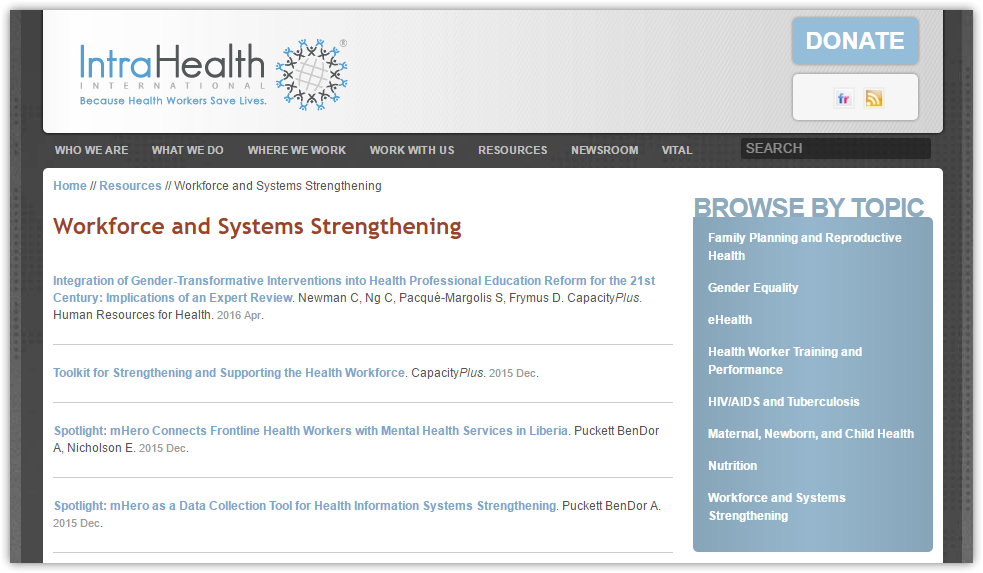
\includegraphics[width=\textwidth]{2016-06-06-Intrah}}

\vbox{
\noindent\textbf{Negatives:}
\begin{itemize}
\itemsep0em 
    \item First off, the page looks like it's a static web page. Because of that, there is no way to filter down results or to add a keyword or date range filter. Someone most likely created the page with the links to items and there's no real way to ``retrieve" something that's outside of the list of links.
    \item There's no way to search only the Resources on the site. I can search site-wide, but if I just want to narrow down the page using a keyword, I'm out of luck.
    \item There's no simple way to determine whether a resource is a peer-reviewed publication, a PowerPoint presentation, or just a link to an external web page. If I'm looking for a specific type of publication, it would take me forever to find it.
    \item The box of links on the right hand side of the page is lacking. It's nice that there is something to better sift through the documents, but when you click on the links, it goes to a relatively unlisted page. There's no indication of where these category pages exist relative to the main list of links. I'm not sure if the page is a completely different set of links separate from the Resources page, or if it's filtering by a tag. My intuition tells me that because the site is static, the links have been added to a page by someone who is writing it by hand. 
\end{itemize}}

\vbox{
\noindent\textbf{Positives:}
\begin{itemize}
\itemsep0em 
    \item The main overview is very clean. It's visually appealing and there's not much to get in the way or make it confusing.
    \item The box of category links is helpful and has obviously been curated for a specific audience or user.
\end{itemize}}

\subsubsection{IntraHealth item page}
\vbox{After clicking on a result, I'm sent to a single item page that displays basic metadata (title, author, etc.) and a link to the external PDF. It's a pretty simple display, but I think that it gets the job done. If you just want to see what they've published, it's in the list.

\noindent
\includegraphics[width=\textwidth]{2016-06-06-Intrah-Item}}

\vbox{
\noindent\textbf{Negatives:}
\begin{itemize}
\itemsep0em 
    \item There is no ``basket" or bookmark feature that would allow users to use a stable permalink to point to the item or page. Even a link to email the publication to yourself would be helpful, but I'm not seeing the feature. 
    \item I didn't see any citation tools that people could use to export the document with metadata. I'm not sure if that is something that users would look for, but I'd like something that creates a permanent link or makes it obvious.
    \item Thumbnails would be nice. If I'm going back to the site to look for new publications, there's no quick way to see if I've previously downloaded the file.
    \item The breadcrumb navigation at the top of the page doesn't point to the correct location when moving up a directory. I clicked ``Browse by Topic" and selected an item from the list, but on the item page, the breadcrumb says that I'm at    \hlbrown{Home // Resources // ITEM} instead of\dots \\ \hlbrown{Home // Resources // Workforce and Systems Strengthening // ITEM}. This is really confusing to me, but I think most people would understand it.
\end{itemize}}

\vbox{
\noindent\textbf{Positives:}
\begin{itemize}
\itemsep0em 
    \item The page is very clean and easy to understand. There isn't anything to get in the way and I don't think anybody using the site would get co;nfused. 
    \item The breadcrumb feature at the top of the page is helpful. Even though it doesn't link properly, I get a basic idea of where I am in the list of information.
    \item Aesthetically, the site is very easy on the eyes. Not too many bright colors or hard lines.
\end{itemize}}

\subsubsection{IntraHealth conclusion}
For the Legal Storehouse, I think that \ul{the visual layout should be simple} and when done correctly, \ul{breadcrumb navigation can help users understand organization}. While Coveo\index{Coveo} will give us more tools and the site will (hopefully) be more complex than what IntraH's got, I think the overall simplicity of IntraH's site is something that I should strive for on the Legal Storehouse site. It looks like IntraH's site needs a dynamic sort feature that programs like Coveo\index{Coveo} offer, but at this time, the static pages are holding them back. The lack of filters on the static page really make it difficult to find what you're looking for. If someone comes into the site looking only for journal articles, they will have to open up each link until they stumble across what they're looking for. For the Legal Storehouse, \ul{the user must be able to quickly locate a specific type of content}. Whether that's a journal publication, PowerPoint presentation, or an external website, there has to be a way for them to locate that material.
\index{IntraHealth@\textbf{IntraHealth}|)textbf}


\subsection{inroads Stigma Resources and Tools}
I then looked at the webpage for inroads\index{inroads@\textbf{inroads}|(textbf}, the International Network for the Reduction of Abortion Discrimination and Stigma.\footnote{Homepage: \url{http://www.endabortionstigma.org/en/Select-Resources.aspx}} I was interested in this site because it's been referred to as the model for what Ipas would like to have on their site. Kyle\index{Goetschius, Kyle} designed the site in javascript to act and look just like Coveo. ``Fauxveo," as he calls it, was designed to replicate the front-end behavior and make it easy for non-technical people to update it in the future. 

\subsubsection{inroads resources main page}
I clicked on the link for ``Resources \& Tools" at the top of the homepage and I was directed to the list of resources.

\noindent
\includegraphics[width=\textwidth]{2016-06-06-inroads}
The page includes a main ``bucket" of results, a search bar to allow searching an index of the entries, and facets on the left side that help narrow down the number of results in the ``bucket." At first look, this is a really slick looking site. I feel comfortable jumping right into the site and using it without having to think about it. 

\noindent\textbf{Negatives:}
\begin{itemize}
\itemsep0em 
    \item There's no way to tell how the items in the bucket are sorted. I think they're sorted alphabetically by title, but I'm not sure. It would be nice to have the ability to reverse the sort direction and to tell the site which columns you'd like to sort by.
    \item There's no icon or other indicator that tells you what kind of document it is. I talk about this in the Conclusion section and I'm not sure if this is a negative, but the fact remains that it's confusing to tell \textit{why} a result is in the bucket when you have two or more facets enabled. 
    \item The ``Not Applicable" Region facet is a bit confusing, bringing up the question as to whether the facets are additive or subtractive. If I don't include that facet, will I miss some items that haven't been tagged with a region? Does that facet mean ``null?" Does that term instead mean something completely different, like ``global" documents that aren't written for a specific location?
    \item The search box does not indicate whether search terms are run against the full text of the items or if it's simply on the metadata. I can see that it's only on the metadata, but someone who might not be familiar with technology might not understand that different. It might be a good idea to tell the user what they are searching.
    \item The metadata information doesn't include full citations, meaning that there's no indication of the author or whether the resource has been published and where. It would be nice if I could search for an author's name in the search bar.
    \item Like in the case with IntraH, it would be nice to export or email a list or ``cart" of articles that I've selected. If I want to generate or save a copy of the citations, I would just have to copy and paste or print the page. 
    \item There's no way to tell whether the linked resource is an in-house publication or if it has been published in an open-access or paywall-ed journal. This goes back to the facet for Type of Content, which I discuss in the Conclusion section.
    \item I'm noticing that the date for most items falls on the first of a month. I'm wondering if this date refers to the date published or the date added to the site. This isn't really clear.
\end{itemize}

\noindent\textbf{Positives:}
\begin{itemize}
\itemsep0em 
    \item I really like the way that the site is organized and how easy it is to get something that you're looking for. The site just works and I don't have to think about how to use it.
    \item The site layout is very clean and I'm not distracted by anything and can focus only on the content.
    \item In a sense, it's no-nonsense and allows people to get what they need without any frills that have the potential to confuse.
\end{itemize}

\subsubsection{inroads item page}
I clicked on a link to an item on the Resources and Tools page and instead of going to an individual item page, it goes directly to the resource. At first, this was confusing, but I got used to it after a few links. Some links go to PubMed pages and others go directly to PDFs.

\noindent\textbf{Negatives:}
\begin{itemize}
\itemsep0em 
    \item There's no way to tell if the link is going to a PDF or to the landing page of a journal. For some links, clicking takes me directly to the resource. Other links takes me to a paywall landing page. Both of these are very different and it would be nice to know which resources are which before clicking.
    \item In my personal experience, this was a bit confusing at first. I was expecting an individual item page to go-between the link to the original document. For some people this could be confusing or it could feel like the site is lacking additional information.
\end{itemize}

\noindent\textbf{Positives:}
\begin{itemize}
\itemsep0em 
    \item This is a no-nonsense way of linking to a resource. If someone is only looking for a specific resource, they can go straight to it once they've located it on inroads' site---there's no intermediary between the two points, making it quicker to retrieve what you're looking for.
    \item I'm sure that this is an easier way to manage and code the project. As discussed earlier, the Fauxveo design was added to overcome budget and time limitations. By adding individual pages for each item, that would have taken more time to create and would require more maintenance as time goes on. As it is now, the team only has to update the main page and doesn't have to worry about each individual page.
\end{itemize}

\subsubsection{inroads conclusion}
One of the interesting things about the site that I hadn't thought about before is that an item that appears in the bucket don't display whichever facets are applied to it. While I can use the facets to narrow down results in the bucket, there's no way to tell for each item what type of content it is without opening it up. I noted this under the ``Negatives" of the site, but looking back, I'm not sure if it's necessary to have all of that information in the item result bucket. Is it important to know all of the information for each document in the bucket? Should the Topic, Learning Agenda Level, Region, or Type of Content tag/label be listed under each item? I'm not sure if all of them need to be listed, but I think it's important to have a few choice ones. At the very least, it would be nice to know the Type of Document for each entry (journal article, opinion piece, etc.). For the Legal Storehouse, I have to \ul{identify which facet labels should appear under an item in the ``bucket"} to make sure it's relevant and helpful without being too cluttered. I'm going to need to get some feedback from Kyle\index{Goetschius, Kyle} on the decisions that inroads made when faced with this problem. Maybe there's a way to only show the labels in \index{Coveo} if you've selected multiple facets. I'll have to check up on that later.

Things are working on the site now with 111 entries, but I wonder if this would be sustainable with more documents. When I'm not able to sort by columns or tell which facets are applied to each item, I think it would be a bit unwieldy to sift through more documents. Additionally, not being able to see the author name of the document is difficult. If I was using the site to locate a specific document, searching by author name would be something that I'd like to do. I think that this site is a great example of how to \ul{organize a lot of documents without overwhelming the user}. While there are some limitations to the site, I think it's very usable and I plan to model a lot of the Legal Storehouse's organization based on the faceted search model. Since Ipas has a similar number of entries, inroads' site organization might work for us. \index{inroads@\textbf{inroads}|)textbf}

\subsection{End of day conclusion}
It's important to note that like the IntraHealth site, inroads had a small budget and their technical limitations must have been difficult to overcome. I think that Ipas' situation will allow me to do things that would have been impossible at either of these organizations. I think that by looking at these two sites, I have a better idea of which direction we're going and I'm aware of a few small things that I'd like to avoid. Moving forward, I'd like to look up some research papers on retrieval, but I'd like to talk to my faculty supervisor first.

I also sent Patty\index{Skuster, Patty} an email asking her if she would be available to meet sometime this or next week to recap what the previous meeting have talked about, update her on the HR decision to pay me for working on the project, and to check in to see if she'd like to add anything to the list of features she would like implemented on the site. 

\vspace{2em}
\noindent
\includegraphics[height=\fontcharht\font`\B]{icons/attachment-email} See Attachment \ref{fig:2016-06-07-Email-Tim-Patty}
\vspace{2em}

\section{June 8, 2016}
I sent an email to Jen Larkin\index{Larkin Rowley, Jen} to follow up with her to see if there were any updates on the Ipas side. Mainly, I wanted to see if I was going to get paid so that I could pay the university for the course. She replied and CC'd Julia\index{Cleaver, Julia} that the issue was taken care of and I just need to code my hours according to a specific work order number. 

\vspace{2em}
\noindent
\includegraphics[height=\fontcharht\font`\B]{icons/attachment-email} See Attachment \ref{fig:2016-06-08-Email-Jen-Larkin}.
\vspace{2em}

\section{June 9, 2016}
I started the day planning to find five journal articles that relate to information retrieval and best practices and take notes on them. I'm going to gather what I can from the CV and other sources I put into a folder on Tuesday (June 7) and I'll do some citation chaining.

I'm still waiting to hear back from Patty\index{Skuster, Patty}. I'd like to follow up with Patty today, but I'm going to send Julia\index{Cleaver, Julia} an email before I double email Patty and potentially overwhelm her. I also checked Outlook and saw her out of office message that says she is in Washington on Thursday and Friday. I may have to wait until next week. Julia sent me an email saying that I should go ahead and email Patty again and specifically ask for a work order number so that I can code it properly on Vega when the pay period ends on Friday (June 10).

I also want to take a look at some more sites to see how they manage their external documents. I'd especially like to take a look at Patty's\index{Skuster, Patty} suggestion to check out the Global Health and Human Rights Database\index{Global Health and Human Rights Database}\footnote{\url{http://www.globalhealthrights.org/}} and see what they're doing. I think RightDocs\index{RightDocs} would also be a good site to look at. They've got a large collection of UN declarations on a huge variety of topics. I'd like to see how they implement facets in their collection. I also plan to look at the way the Legal Storehouse currently works on the Ipas website. I've been in a couple of meetings with people and I've received a lot of feedback about it, but I think it's important to put it into writing so that I have something to look back to later on in the project.

\subsection{Global Health and Human Rights Database}
\index{Global Health and Human Rights Database@Global Health and Human Rights Database|(textbf}
At the first meeting of the project, Patty\index{Skuster, Patty} suggested that she really liked the layout of this site. She suggested that I take a look at it to see if we can implement anything like it for the Legal Storehouse. 

\noindent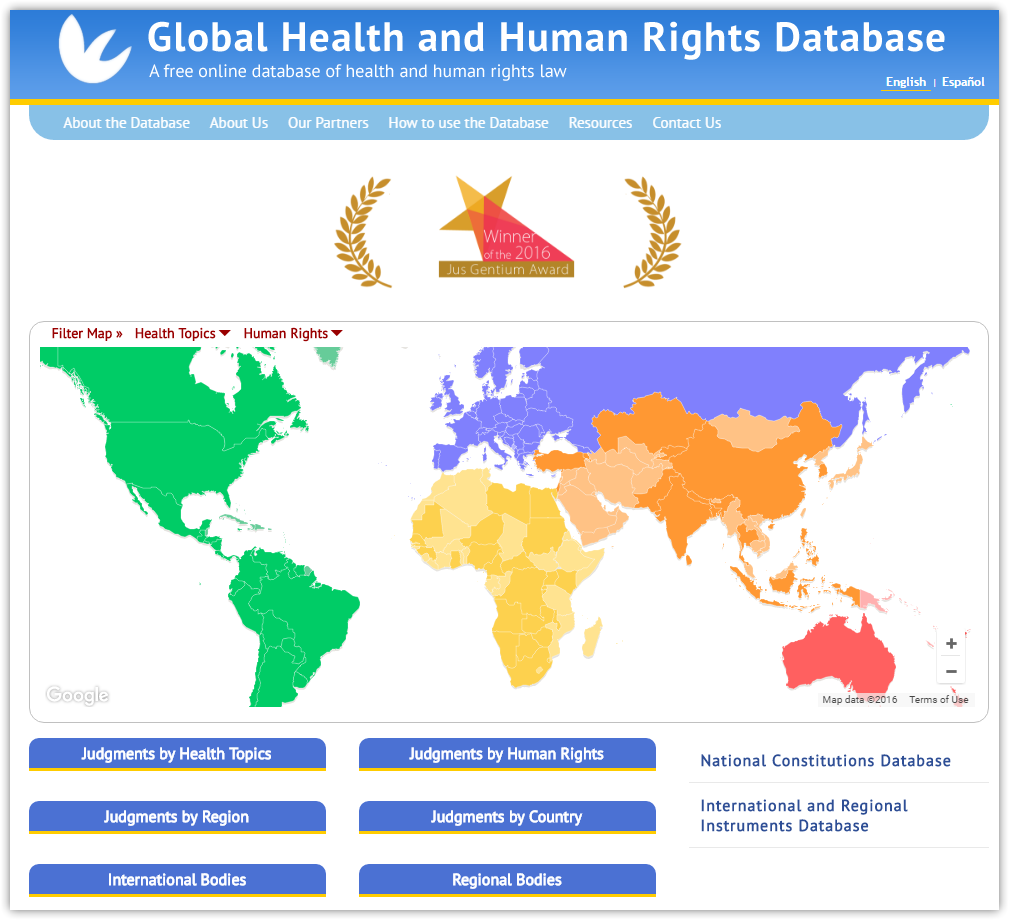
\includegraphics[width=\textwidth]{2016-06-09-Global-Health-Main}

The map on the main page was interesting and I could see how it could be useful, but I don't think the Legal Storehouse has enough country-specific documents to populate the map. Most of the items are global or don't specify the country 

\subsubsection{Global Health and Human Rights Database category view}
\noindent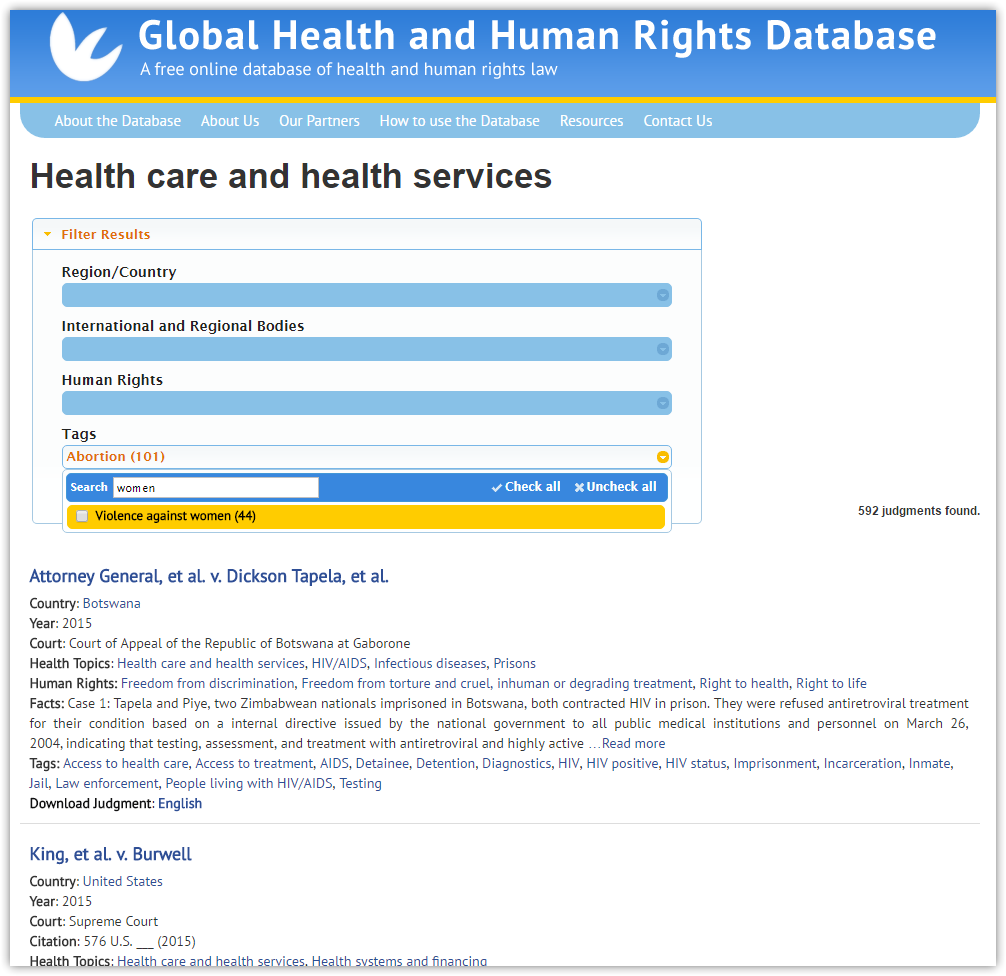
\includegraphics[width=\textwidth]{2016-06-09-Global-Health-Categories}

\noindent I clicked on a category and was directed to a page with about 592 items. There is a ``Filter Results" box at the top that I clicked to open up a series of facets. I played around with them a bit to find out the functionality of the site and to see how the items in the bucket can be manipulated.

\noindent\textbf{Negatives:}
\begin{itemize}
\itemsep0em 
    \item I don't see anywhere to search the resources from the main page of the site. There doesn't seem to be a way to just type in what you're looking for. This could be frustrating for some people who are looking for a specific title or citation.
    \item I clicked on a category, but I don't see a way to quickly change categories or to change the view to see items that might fall into multiple categories. There really is no way to navigate to other categories or to understand the relationship between them from the top navigation page. I can do this on the items in the list, but it would be nice to have that control at the top.
    \item There is now way to re-sort the items on the page. They're sorted by date and there's no way to change that. It was frustrating to me and I would imagine that you'd have to scroll through the entire list if you're looking for something specific. 
    \item  I wasn't able to limit the date that things were published/released.
\end{itemize}

\noindent\textbf{Positives:}
\begin{itemize}
\itemsep0em 
    \item The design is really clean and straightforward. While it looks a little different than the layouts that I'm used to, I think that it does a good job of displaying and organizing the documents without cluttering up my view.
    \item I also really like how the items have links to subtopics right on the main view. I can easily find similar documents by clicking on these links. I think that I could implement something like this for the Legal Storehouse.
    \item In the filter settings, each facet drop down button has a search bar that I used to find specific tags. This is really helpful and was much more usable than just having a huge list of tags to choose from. This is a really cool feature and it was really useful to me and I found a similar option on the RightDocs\index{RightDocs} website.
\end{itemize}

\subsubsection{Global Health and Human Rights Database item view}
\noindent I clicked on the title of an item and I was redirected to a page of metadata with tabbed sections. There are also links to related judgments at the right pane. The link ``View full summary and print" brings up a window with the full metadata information as an HTML page. ``Download summary as PDF" serves up the same information as a PDF.

\noindent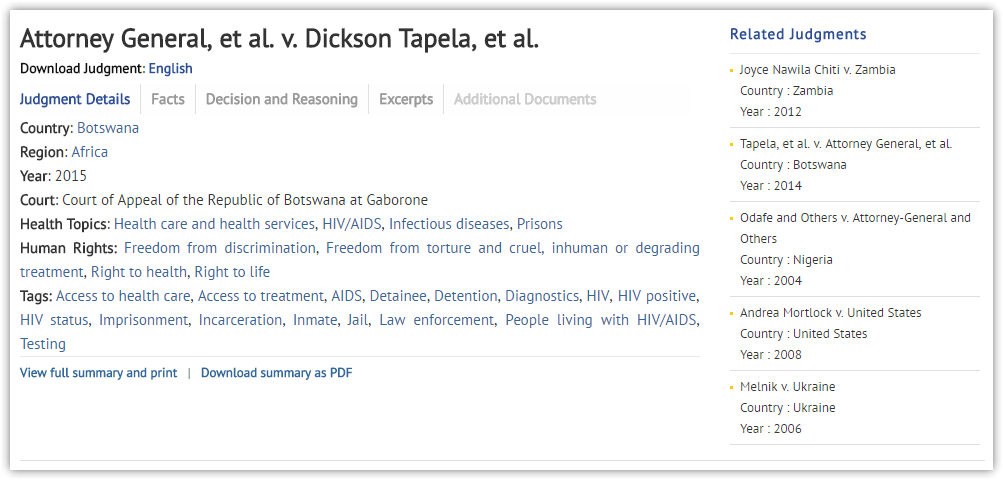
\includegraphics[width=\textwidth]{2016-06-09-Global-Health-Item}

\noindent\textbf{Negatives:}
\begin{itemize}
\itemsep0em 
    \item Some people could be confused by this intermediary item page. It might be easier and more straightforward to link directly to the resource like other projects have done.
    \item I'm sure that the metadata and numerous pages are difficult to keep up to date. It would be easier if the item pages didn't exist.
    \item The tabs at the top of the item page may be confusing to people who aren't familiar with this type of navigation. It may be better to just have the full summary as the default view.
    \item The ``Download Judgment" button isn't where I expect it. I would think that it would be next to the download summary links. The current position may be confusing to some people.
\end{itemize}

\noindent\textbf{Positives:}
\begin{itemize}
\itemsep0em 
    \item The layout is really slick and I love the way that everything is organized. It looks great and from the first glance, I can really get a good idea of what I'm looking at.
    \item The ``Related Judgments" panel at the right side of the item view is also really helpful. I could see this really coming in handy when doing research on a specific category. Now that I think about it, I don't know how this list is populated. Surely it can't be a hand-picked list. There has to be an algorithm used to find related documents. I wonder if I can replicate this. 
    \item The tabs offer a better way to view all of the information. If they were all displayed at once, it might be overwhelming. The way its displayed now makes for a great experience.
    \item The Excerpts tab may be exactly what we're looking for in the Legal Storehouse. It's tucked away so it's not glaring at you and distracting, but it's still accessible if you're looking for it.
\end{itemize}

\subsubsection{Global Health and Human Rights Database conclusion}
This site has a lot of great resources and I can see why Patty\index{Skuster, Patty} likes the way they're organized. Once you've found a judgement, it's easy to locate similar items by clicking on their tags. In this case, the tags work nicely because all of the items in the database are of the same type---there's no need to filter out peer-reviewed articles, opinions, etc. because the metadata \textit{is} the most useful document and the judgement is just a PDF. I think that the tabbed view adds to this organization and is a great model for how I'd like to do quotes on the Legal Storehouse. I think it's important to \ul{keep excerpted passages and snippets}, but \ul{move them to another area}. I think that if someone is interested in reading the snippet, they will do so. We shouldn't serve up a snippet on the main category view.

That being said, while it's easy to locate other documents \textit{after} you've found the one you're looking for, getting to that initial judgment or finding a specific one might be difficult. The site doesn't offer any type of keyword searching or filtering that can assist users in finding what they need by searching all of the entries. I think for the Legal Storehouse, it's imperative that we have a \ul{search box} that can filter out \ul{indexed item metadata} for the entire site so that users can find things they're looking for in addition to being able to filter through the items in the bucket. While this may seem like an easy thing to do, I'll have to \ul{decide whether we're also going to include the full text in the index or just the metadata}. In either decision, I have to \ul{make it evident to the user which one they're searching through}. 
\index{Global Health and Human Rights Database@Global Health and Human Rights Database|)textbf}

\subsection{Ipas Legal Storehouse}
I wanted to also look at the Legal Storehouse as it currently is and give an overview of what works and what needs to be changed. I've met with people at Ipas several times to go over the site and each time, people have expressed similar frustrations with the layout and the accessibility of it. 

\noindent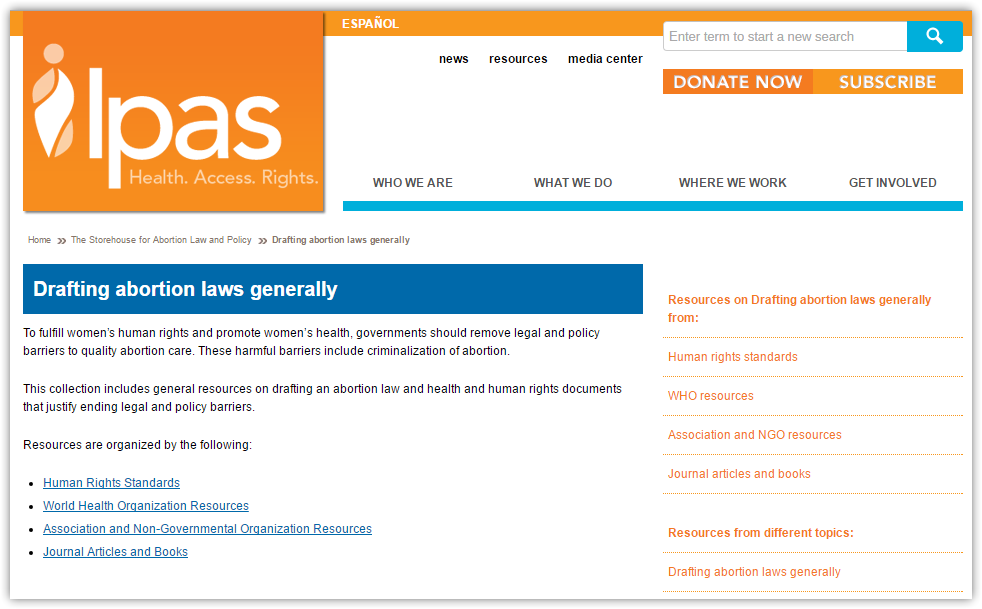
\includegraphics[width=\textwidth]{2016-06-09-Ipas-landing}

\noindent This overview may be a little bit more complicated than the previous ones because the site is difficult to navigate. It's organized with a main category or ``Resource topic" landing page and four sub-pages that are divided by origin or publication type (e.g. peer-reviewed article, corporate author). 

\subsubsection{Ipas Legal Storehouse main page}
After clicking on a category and getting to the landing page, I then clicked on the ``From" limiter to specify the origin or type of documents that I was requesting. I was directed to another static page with a list of links to other resources.

\noindent
\includegraphics[width=\textwidth]{2016-06-09-Ipas-category}

    \noindent\textbf{Negatives:}
    \begin{itemize}
    \itemsep0em 
        \item First of all, the site is very difficult to find. From the Ipas homepage, I had to navigate to \hlbrown{Home $\rightarrow$ What We Do $\rightarrow$ Advocacy $\rightarrow$ Human Rights, Laws and Policies} and clicked on a link in the panel at the right of the page. I got frustrated at one point and just Googled ``Ipas Legal Storehouse" and found the page that way. I really wish it was easier to find the main page for the Storehouse.
        \item The navigation bar at the top of the main page for the Legal Storehouse isn't correct. Even though I navigated to the page from a page under Advocacy, the breadcrumbs note that ``Home" is the previous page. This can be disorienting for anyone who visits the site and I certainly didn't understand it.
        \item Just by looking at the page, I can tell that it's a static page with links to item pages. Because it's static, there are no tools to sort, filter, or search through the results. The only thing I can do to locate more articles is to click on another category on the right side of the page, but there's no way to tell which category the individual items fall into. This was really disorienting for me. 
        \item I wanted to count how many unique items there were on the site, but I wasn't able to figure it out. I think there are quite a few items that have entries on multiple category pages, but the tags/labels that have been applied to the item aren't visible (or do not exist). I'm not able to tell which articles are tagged with multiple topics.
        \item The snippet of the document in the metadata on the item is confusing. I understand why some of the things have been highlighted or bolded, but I don't understand how that fits into the overarching category or topic. I'm sure there's a reason for it, but I wish it was explained somewhere.
        \item Although the resources are divided up by type or origin, there's no way to tell if the item that I'm clicking on is a PDF or a different format. There are some links that go to web pages and others that go directly to PDF files. 
        \item The menu on the right side of the page to filter by origin or author is confusing. It was difficult to know that the menu just appears on top of the topics menu when you click on a topic. I might have missed it on my first time. It needs to be more prominent or act as a sub menu. 
        \item I'm also noticing a few of the links are broken and aren't going to the correct link. I'm sure this would be frustrating for anyone using the site.
    \end{itemize} 
    
    \noindent\textbf{Positives:}
    \begin{itemize}
    \itemsep0em 
        \item The collection of documents is curated and has been hand-written by someone. This goes for something in that the information that is pasted or written in with a lot of thought for its order on the page, the categories it falls into, and which words are highlighted in the full-text snippet.
    \end{itemize}

\subsubsection{Ipas Legal Storehouse item page}
After I clicked on an item on the main page, it goes straight to the linked resource. Sometimes it goes directly to a PDF and sometimes I'm linked to a landing page for a publisher. This behavior is very similar to the inroads\index{inroads} site that I looked at yesterday. The positives and negatives are the same for this behavior on the Ipas website.

\subsubsection{Ipas Legal Storehouse conclusion}
Firstly, I think \ul{the Legal Storehouse needs to be easily accessible} coming from external websites or the Ipas main page. It should be a lot easier to find and people shouldn't have to search Google to see it. I don't know much about driving traffic to websites or how to increase the number of ``clicks" something gets, but I'd really like to see the project be of use to someone. At the very least, I'm going to request that we \ul{add a link on the Ipas homepage} so that people can find it easier on the website. I'd also like to \ul{fix the breadcrumb navigation} so that people understand where the project is located on the Ipas website. If possible, I'd also like to \ul{add some SEO tags to make it easier to find through a search engine}. It would be cool if people would find the project without first knowing it or Ipas exists.

After the accessibility factor, the broken links were the most frustrating part of the site. When I found something that looked interesting and tried to open it, it wouldn't be available. I think that this could be remedied if there was a way to link to a stable \href{http://archive.org/web/}{Archive.org} or \href{http://archive.is/}{Archive.is} link. Better yet, if we could host the PDF on the Ipas servers, we could avoid ever losing the document. I'm not sure I'll be able to store copies on our server, but in any case I need to \ul{fix broken links and find a solution for long-term access}.

I think that while this is a good collection of items and that the information is crucial for users, the way it's displayed isn't great. I've been to the site quite a few times, but I'm still confused by the way the documents are organized. I see now that each category on the right side also has four sub-pages divided by origin or type, but it took me longer than necessary to understand that connection. I think I need to \ul{avoid using sub-pages} and instead \ul{keep everything in a single bucket} that has tools I can use to filter items. 

\subsection{RightDocs}
RightDocs\index{RightDocs@\textbf{RightDocs}|(textbf}\footnote{\url{http://right-docs.huritech.org/}} is a new website that allows people to search and filter through Human Rights Council resolutions. At the time I'm writing this note, it has over 1,200 documents. It was a little difficult to get access to this site. I had to submit my email address and confirm it, but eventually I got in and was able to access the site. Immediately upon entering the site, I'm presented with a list of documents. There's no landing page, but the email confirmation I received explains the rationale behind the site and how to use it.

\subsubsection{RightDocs main page}
The main page is straightforward and has a listing of all of the items in a large ``bucket." Towards the top of the page, there is a tool bar with filter options and navigation bar at the very top with a search box that searches metadata and full text. There are also a few links at the top of the page to display categories of Resolution, specific Reports, and specific States. Also, there's a pane on the left side of the page that allows users to add specific states to compare their voting history. I notice that as I add filters from the top menu, they appear on the left panel.

\noindent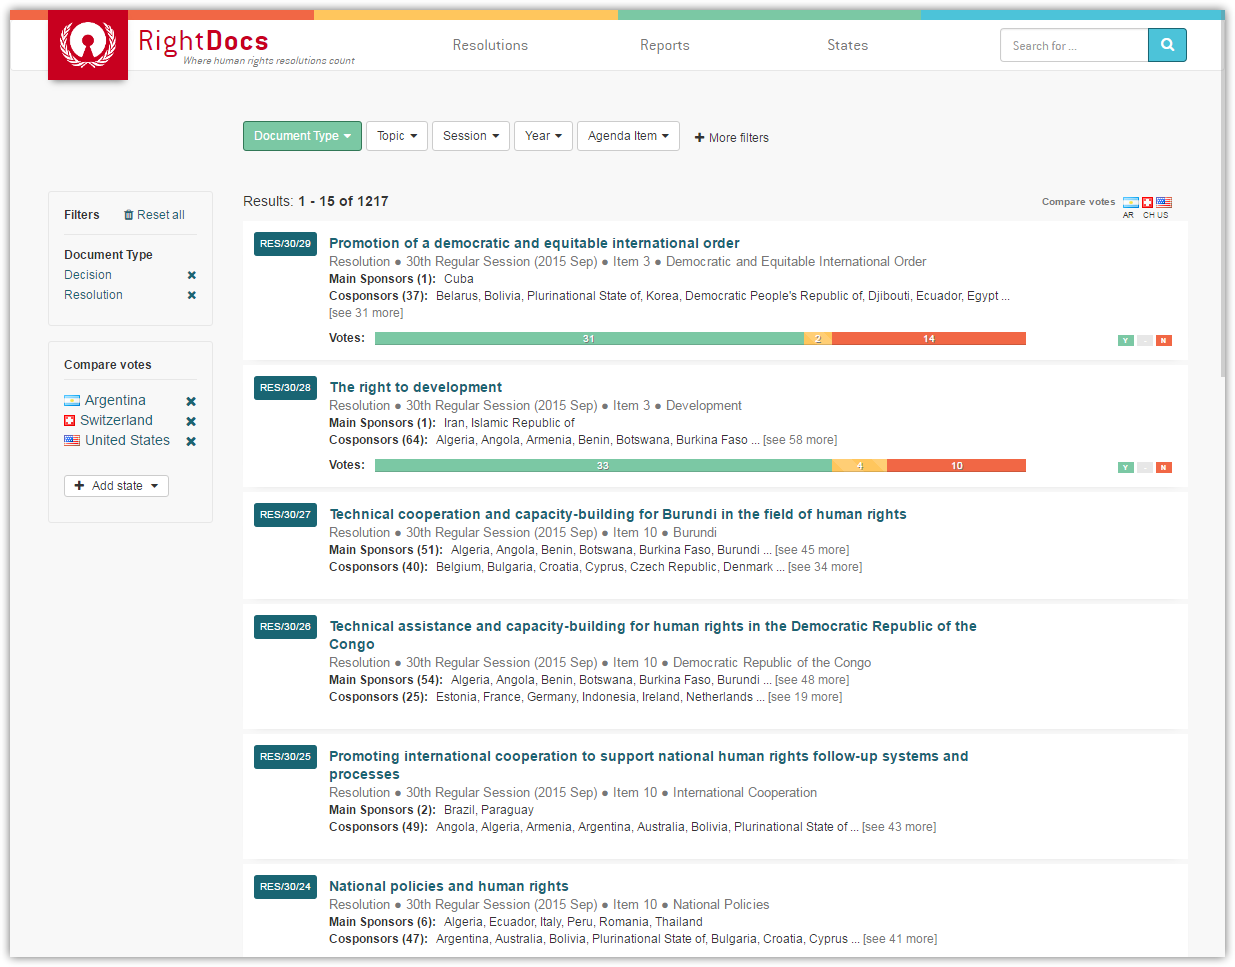
\includegraphics[width=\textwidth]{2016-06-09-RightDocs-Main}

\noindent The filter dropdown menus have the option to search for tags and to change the sort direction and toggle AND/OR boolean modes.

\noindent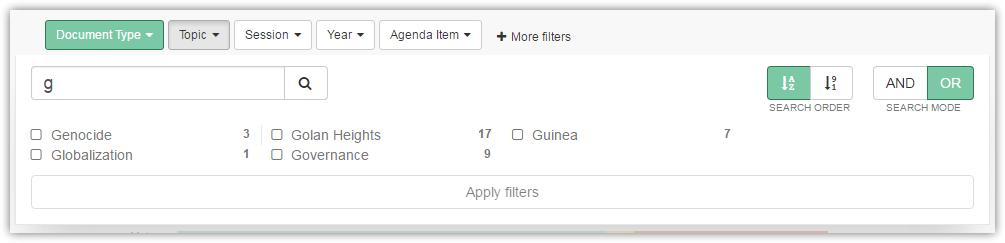
\includegraphics[width=\textwidth]{2016-06-09-RightDocs-Filter}

\noindent\textbf{Negatives:}
    \begin{itemize}
    \itemsep0em 
        \item This site may be a bit overwhelming to people who aren't savvy with this level of complexity. I think that while the search box is great for people to quickly locate something, the ability to search within tags and control facets with that level of granularity can be too much control for some people. 
        \item I'm not sure if the ``Votes" graph is needed. I think that for many of these resolutions, the comments and statements by the states are more complicated than the vote count. It looks nice, but there might be more important information to display in a graph than just Yes-No tallies.
        \item The ``Year" facet could be improved. The years are displayed as tags and can be a bit confusing and/or frustrating to select multiple boxes if you're just looking for a span of years. It would be nice if you could just type in a range or use a slider to select a range of time.
    \end{itemize}
    
    \noindent\textbf{Positives:}
    \begin{itemize}
    \itemsep0em 
        \item The overall layout of the site is really easy to understand. The colors aren't too overwhelming and I feel like I can jump right in without thinking about how to use the site.
        \item The filter bar at the top of the page is deceptively chock full of features. While it may seem like there will only be a drop down with a simple list when you click on ``Document Type," ``Topic," or other facet, the drop down menu has several great sorting features that allow me to filter down the items in the bucket without issue. 
        \item Again, going back to the filter bar, I really like the way that I can search for terms within a specific facet instead of just selecting from a list. For example, in the ``Topic" facet, I can sift through the huge list of tags, or I could just search for what I'm looking for. This is extremely useful for cutting down retrieval time. 
        \item The ability to change the search mode and the order of the results within the search bar gives users a lot of control over the results. This filtering behavior is really powerful and I think once people get the hang of it, they'll feel comfortable with it.
        \item While I noted the ``Year" facet has negative behavior in the previous section, I think that, in a way, the ability to select specific years actually improves the control that users have. For example, if you're just looking for the years 2011 and 2013 and want to skip 2012, the way that the facet is handled now gives you the ability to do that. I'm not sure how often someone would need a feature like this, but it could be useful to maybe have all three options to give people a choice.
        \item The ``Search" box allows you to search the entire site---metadata and complete full-text. Also, this website has one of the best search interfaces in that it displays the results with the term highlighted.
    \end{itemize}
    
\noindent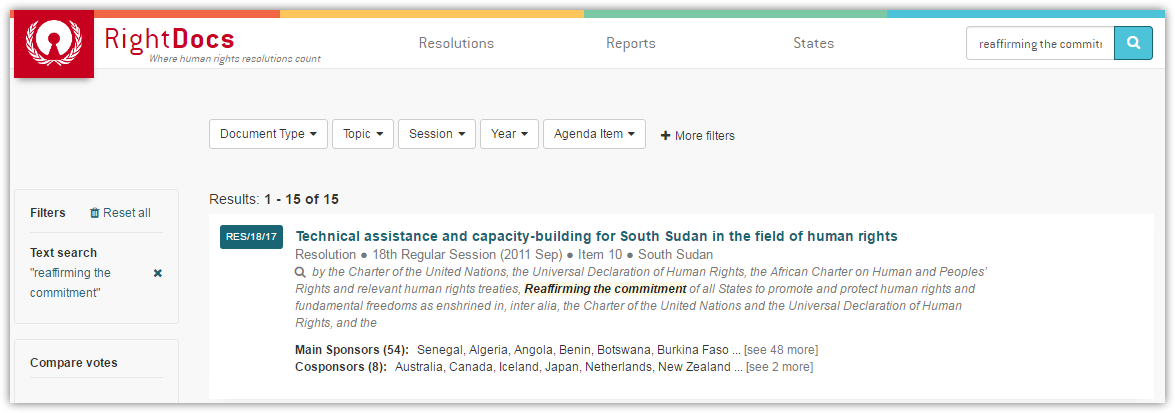
\includegraphics[width=\textwidth]{2016-06-09-RightDocs-Search}
    
\subsubsection{RightDocs item page}
After I clicked on a title from the main page, I was directed to an item page. The page has a panel on the left with a link to the original document as an HTML or PDF file. Additionally, the item has metadata and includes a list of sponsors and the voting history. On the main part of the page, it has the full-text of the resolution.

\noindent
\includegraphics[width=\textwidth]{2016-06-09-RightDocs-Item}

\subsubsection{RightDocs conclusion}
I think that RightDocs offers a lot of power to people who are trying to sift through a large number of documents. It's got a lot of tools, but at the same time, isn't too confusing. I felt right at home.

For our Legal Storehouse, there's a lot that I'd like to implement from RightDocs. I think it's necessary to \ul{put the search bar on the main page, not behind a menu}. For people to feel comfortable with the site, they should be able to search the metadata of every item to find what they're looking for. As I've said before, I'll need to determine what's searched, but I think \ul{the text on each item that's visible on the category page should be searchable}. I also think that for facets that have a lot of tags, we should \ul{implement a small search box for each facet}. That way, users can quickly locate the tag that they're looking for.\index{RightDocs@\textbf{RightDocs}|)textbf}

\subsection{Research articles}
In her article, \citet{Kelly2009} defines an evaluation of information retrieval with the question, ``Does this system retrieve relevant documents?" \citep[p. 2--3]{Kelly2009}. \todo{Finish transcribing notes here.}

\section{June 13, 2016}
\subsection{Issues with Ipas work order and time sheet}
Patty\index{Skuster, Patty} emailed me back with the work order. 

\vspace{2em}
\noindent
\includegraphics[height=\fontcharht\font`\B]{icons/attachment-email} See Attachment \ref{fig:2016-06-13-Email-Patty}
\vspace{2em}

Meanwhile, I emailed Julia\index{Cleaver, Julia} because I was having an issue with my time sheet. For some reason, I was only able to edit one day. She checked with HR and it looks like my contract renewal wasn't inputted into Vega, so I wasn't able to edit anything after May 20th. HR fixed the issue and I was able to edit the line for R\&E, but I still wasn't able to edit the document for ``Legal and HR'' to input my Field Experience time. 

\vspace{2em}
\noindent
\includegraphics[height=\fontcharht\font`\B]{icons/attachment-email} See Attachment \ref{fig:2016-06-13-Email-Julia}
\vspace{2em}

\subsection{Check-in meeting with Katrina}
I met with Katrina\index{Lee, Katrina} to talk about my competitive analysis\index{competitive analysis} and to discuss this document (that you're holding now). She's pleased with the work I did and encouraged me to now begin going through all of the documents to find common categories and tags that can later be used as facets. She recommended that I put the item metadata/information in a spreadsheet that can be later turned into a schema. 

Additionally, she recommended that I check in with Patty\index{Skuster, Patty} and maybe give her a copy of these notes. I'm waiting for her to get back from Washington, and then I'll follow up with her for a quick check-in meeting.

\section{June 14, 2016}
\subsection{Creating a spreadsheet from the Legal Storehouse website}
I started the day with the goal of creating a spreadsheet from all of the entries on the Legal Storehouse page. I think this will take a long time, but it's mostly copying and pasting, so it's not going to be terrible. I also have to think about which metadata things I want to preserve, so I've got a lot of work ahead of me. I don't know if date and author are appropriate and I don't know if I should just leave the stuff as-is and add information later.

\section{June 16, 2016}
\subsection{More spreadsheet work}
I started the day with the goal of auditing all of the links on the spreadsheet. This took some time, but I was able to check whether the links resolve or not. I also tried to fix the links if they didn't resolve. This issue brings up the conversation of how we deal with link preservation. I wonder if I should be using \href{http://archive.org/web/}{Archive.org} or \href{http://archive.is/}{Archive.is} or some other type of link archiving website. 

\section{June 20, 2016}
\subsection{Timesheet coding}
Julia\index{Cleaver, Julia} talked to me this morning and explained that I should just go ahead and submit my timesheet with the hours billed to the regular Library line. She said that for some reason, Vega doesn't play nicely with employees working for two different job classes. In this case, since I'm the student, they can't also record time for Consultant pay. After I submitted the timesheet for this week, however, she mentioned that next time I should bill under the Unrestricted Policy line at US-1080-1013.
\subsection{Findability presentation by Katrina}
Katrina\index{Lee, Katrina} gave a presentation on findability to several Ipas employees. Findability\index{findability|textbf} involves SEO, accessibility, and wayfinding\index{wayfinding} and is a metric that can be used to measure how easy it is for people to find what they're looking for on your website. In the presentation, she talked about ``semantic HTML\index{semantic markup!HTML|textbf}," a concept that she defined as, ``using HTML to reinforce the structural meaning of the information \dots rather than just defining presentation and look." Additionally, wordiness can detract from the effectiveness of a page and can hinder its findability. \todo{Add more information about its applicability to the project.}

\section{June 21, 2016}
\subsection{More spreadsheet work}
I continued working on the spreadsheet today. I made sure that all of the links are resolving and that the entries are all unique. I made sure that I preserved the notes and ``from" and ``topic" lines to make sure that we're not losing the relevant quotations from each topic. There were some articles that were in five different categories and many of the entries were duplicates, but had slightly different spellings and abbreviations. This made the process a little difficult and time consuming to find unique entries. I also had to make sure that the unique entries were saved with each of the duplicates' topics. 

\section{June 22, 2016}
\subsection{Short meeting with Julia}
I talked to Julia\index{Cleaver, Julia} about how we can preserve the PDFs for long-term use. She suggested that for most of the publications from the WHO and other open-access sources, we can add the document to the catalog and provide a link from Venus that will be available externally. This will allow us to have the document in our catalog so that we can keep track of it, while ensuring that the document will be available over the long term. She recommended that I bring this up with Katrina next time we meet (probably Monday, June 27, 2016).

\section{June 28, 2016}
\subsection{Working from home}
I worked from home today. I wanted to make sure all of the items in the spreadsheet have been cataloged so I checked InMagic\index{InMagic} to see how many are. Many aren't, so I began the process of cataloging them and adding them to Fulltext. I also changed some of the author and title information in the spreadsheet to reflect the correct information in the catalog.

\vspace{2em}
\noindent
\includegraphics[height=\fontcharht\font`\B]{icons/attachment-email} For the current spreadsheet layout, see attachment \ref{fig:2016-06-28-spreadsheet}.
\vspace{2em}

% \subsection{Julia's stepfather}
% I was just notified that Julia's\index{Cleaver, Julia} stepfather has passed away this morning. I'm so sorry for her loss and I hope she is doing well. She plans to be out of the office for the remainder of the week.

\section{June 29, 2016}
\subsection{Skype for Business meeting with Katrina}
Katrina\index{Lee, Katrina} and I met today over Skype for Business and I explained some of the stuff that's in the spreadsheet. Overall, she was pleased with the spreadsheet and recommended a few changes to improve its usability. Namely, she recommended that...
    \begin{itemize}
    \itemsep0em 
        \item I need to \ul{add a field for the journal articles to see if they're peer-reviewed}. We're not sure if all of PubMed\index{PubMed} is peer-reviewed (particularly theses) so we'll have to check with someone in the Library to make sure. Katrina\index{Lee, Katrina} explained that for the people coming to the site, we need to explicitly display whether the article is peer-reviewed so that they can use it. Without this, they might not trust the source and may skip it over.
        \item There are a lot of confusing names in the spreadsheet and many of them are complete citations. I need to \ul{rename each entry to something that makes sense}, \ul{create a column for citation information}, and \ul{move that citation information from the name to the new column}. Katrina recommended that I use APA styling to create this. We might be able to use BibTeX and allow Coveo to export to a citation style, but I'm not sure if it has this capability.
        \item I need to \ul{send Patty an update of what I've currently been working on} and see if she has any recommendations for work going forward.\index{Skuster, Patty}
        \item I need to \ul{remove all of the Venus links from the default URL field} and \ul{replace them with external links}. They're fine in the cataloged field, as per my discussion with Julia\index{Cleaver, Julia}, but they won't be available to anyone outside of our intranet. In many cases, the ones with Venus information \st{are} should be available on the Ipas website.
\end{itemize}
Katrina\index{Lee, Katrina} will set up a meeting with Kyle\index{Goetschius, Kyle} in the upcoming week to discuss Coveo\index{Coveo} and SiteCore\index{SiteCore} stuff. She expects that the spreadsheet should be very useful when we get the correct fields set up in SiteCore\index{SiteCore} and that most of the technical work will go along smoothly. She will schedule the meeting and get back to me via email.

\section{July 1, 2016}
\subsection{Sakai post}
For the first Sakai assignment, I was asked to respond with a quick summary of my work and to explain any obstacles or deficiencies in my site.

\begin{displayquote}
As you respond to this thread, please introduce yourself to the group, and let them know where you are spending your Summer FE.

This seminar was designed to offer students currently participating in a Field Experience to have an outlet to discuss how to integrate their academic course work and theoretical knowledge within a practical work setting. 

Let's begin thinking about this integration between theory and practice. 

1) What SILS classes (or topics covered within classes) have been the most beneficial to your progress during your field experience?

2) What have you noticed while working at your site that you wished you HAD covered in your coursework?

Sometimes this integration is seamless, but more often there are some barriers that emerge that can impact completing your learning objectives, developing a meaningful professional development experience, and creating opportunities for mentorship.

The goal of the FE seminar is to not only unearth these potential barriers, but offer constructive strategies for moving past them.

1) What barriers have you already experienced at your site? 

2) What kind of barrier was it ~ communication issue, lack of technical expertise, not connecting with your supervisor and/or colleagues, needing to realign your learning objectives, or other area for concern.

3) Have you removed the barrier, and if so, how?
\end{displayquote}
\noindent My response was...

\begin{displayquote}
Hi all! I'm Tim and I'm a second year MSLS student. I'm currently working at Ipas to redesign their Legal Storehouse. Ipas is an international NGO that works to improve women’s health and protects access to safe reproductive health services. The Legal Storehouse is a website with a bunch of great documents that can help people at other organizations write policies for their organization. While it's got a lot of curated information, there's absolutely no way to access them. The current site is a collection of static web pages that have been transferred from a Wordperfect document. I'm tasked with migrating the existing information, cleaning up the metadata, developing a taxonomy for the project, and creating a new set of entries from this information. SiteCore and Coveo will be the backend and frontend, respectively, and I have just begun working with JSON.

I took ``Information Access for Underserved Populations'' with Cliff Missen last fall. One of the many things that I learned in the course was how unreliable and often overpriced internet connections can create huge gaps between countries and groups of people. Cliff reiterated that information gaps lead to tangible differences in health care, political activism, and in overall quality of life, among other issues. I began the Legal Storehouse project with that information in mind. In the implementation phase, I will push for low bandwidth requirements and to meet other needs that workers in developing countries are asking for. Another class I took was “Organization of Information” with Robert Losee. I wish I had learned more about measuring information retrieval in that course and I feel it’s something that’s important to what I’m working on. I’d like to be able to understand and track how quickly someone can retrieve what they’re looking for and be able to tweak the web interface and backend accordingly. If I had these skills, I might be able to improve my current work processes in anticipation for maintenance and the analytics schedule I will work out with my site supervisor. At the moment, I will most likely need to talk to my faculty supervisor about best practices for this, but I really wish I learned more about it in class.

I really enjoy working with everyone at Ipas. It's a large organization internationally, but in Chapel Hill, there’s a tight knit group of people who are dedicated to protecting women’s health and facilitating knowledge sharing. The barriers that I've encountered over the past few months couldn't be avoided and I've learned how to overcome them through learning how to anticipate other people’s time commitments, work loads, and other various limitations that may have an impact on my ability to get things done. It would be great to think, ``We can have this goal done in a week!'', when the reality is that many people are working on many different projects and don’t have my deadlines at the top of their to-do list. I think this is a great reality-check for me to learn what it’s like to work in a big office and how to juggle a lot of responsibilities and work relationships to make sure the project reaches completion.
\end{displayquote}

\section{July 6, 2016}
\subsection{SiteCore meeting}
I met with Katrina\index{Lee, Katrina} and Kyle\index{Goetschius, Kyle} to talk about SiteCore's\index{SiteCore} features and what I can expect when I start working with it. It was informative and a lot of it overlapped with the meeting a few weeks prior where they demoed some of the features of the backend of SiteCore\index{SiteCore}.

\section{July 11, 2016}
\subsection{Meeting with Katrina}
I met with Katrina\index{Lee, Katrina} this morning to update her on the spreadsheet and also to start looking at SiteCore\index{SiteCore}. From the tour I took, we're going to need to create a metadata template that we can use to insert into pages. The items that I create will use the metadata template. I think that's how it works.

I think that I'll understand the connection between the templates, pages, metadata, and entries once I get access to SiteCore\index{SiteCore} and have the ability to play around with some of the content. As of right now, it's more conceptual. I'd like to get access as soon as I can so that I can start with some of the metadata stuff.

\section{July 12, 2016}
I started the day with the plan to jump right into the mockups. I need to find a program or website that works for my project, is easy to use, and can be shared with other people. Once that's done, I need to create something that models how the site will look in the end and explain how each of those parts will behave. Katrina\index{Lee, Katrina} and I will then turn this mockup into a template for SiteCore\index{SiteCore} to be used in pages. I'm not 100\% sure how SiteCore works, but I'm sure I'll get the hang of it once I get a login and have the chance to play around with it a little.

\subsection{Site mockups}
I started the day with the intention of creating a wireframe mockup of how I want the Legal Storehouse to look. Per Katrina's instructions, I looked at several different solutions (PowerPoint, Visio, Balsamiq) and I found that the \href{http://draw.io/}{Draw.io}\index{draw.io} web app is the best solution for what I want to do. I created a basic mockup of the site and started defining and explaining how things will work on the different parts of the site. It looks pretty rough and it's a bit cumbersome to get get everything organized so it's easy to understand, but I think it'll be better if I keep playing with it.

\subsection{Cataloging}
I'm going to continue working through the resource list to catalog everything. There's still about 75 sources that need to be cataloged, so I have my work cut out for me!

\section{July 15, 2016}
Today, I wanted to finish the mockup and polish some of the rough edges, but most of my day was spent doing other library tasks. A reference/research request came to the inbox and was directed to me. Additionally, a long list of requested documents was also routed to me. I found most of them, but I had to go to the Health Sciences Library at UNC to scan two of them. This took most of my time.

\subsection{Mockup work}
One of the biggest conceptual issues that I came across was how I would display the search results in relation to the filtered categories. The original Legal Storehouse webpage organizes the entries by category and each entry has a summary or blurb that explains its relevance to the category. This makes sense in that layout, but in the new ``bucket" layout, I need to find a way that will selectively highlight or display the search results in relation to the selected category. I'm not really sure how this works, so I think I'm going to look back at the sites that I did the comparative/competitive analysis of. When I find something I like, I'll add it to the mockup and explain how each part works.

\vspace{2em}
\noindent
\includegraphics[height=\fontcharht\font`\B]{icons/attachment-screenshot} See mockup screenshot as Attachment \ref{fig:2016-07-15-mockup}.
\vspace{2em}

\subsubsection{inroads}

\begin{center}
\noindent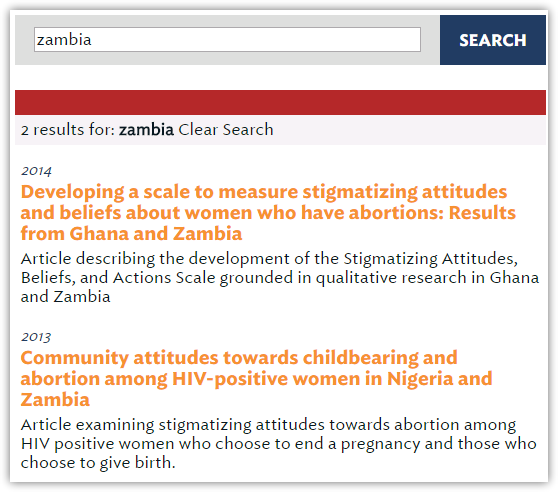
\includegraphics{2016-07-15-inroads}
\end{center}

I tried a simple search on the inroads\index{inroads} website to filter out some results and see how the site displays the search terms in the ``bucket." From what I could see, the results are not highlighted and it was difficult to see how my search terms related to the list of results. Again, since this is a static site, there's really not much they can do with selectively displaying the facets in relation to the search term, but there should be a way to highlight the search terms in the results. In any case, inroads is missing this feature, but since the description is short and there aren't too many entries, it works. I think it would be disorienting if there were more entries, but for what they've got on the site, it's fine. One thing I did like, however, was the way that the site displays both the search term and the selected facets at the top of the results list (image shown below). I'd like to implement something like this on the Legal Storehouse so that it's obvious how the search terms relate to the facets. Additionally, there is no way to determine what facets each item has. When I select ``Stigma" as a facet, it's easy to deduce that the list of results all have ``Stigma" as their topic. When I select multiple facets, however, there's no way to determine whether the facets I've selected are exclusionary, meaning the site will only display results that have both facets, or inclusionary, meaning it will display results with either facet. Allowing the user to see which labels have been applied to each item would make it much more clear to the user why an item shows up in the results list.

\noindent
\includegraphics[width=\textwidth]{2016-07-15-inroads-facets}


\subsection{RightDocs}
\noindent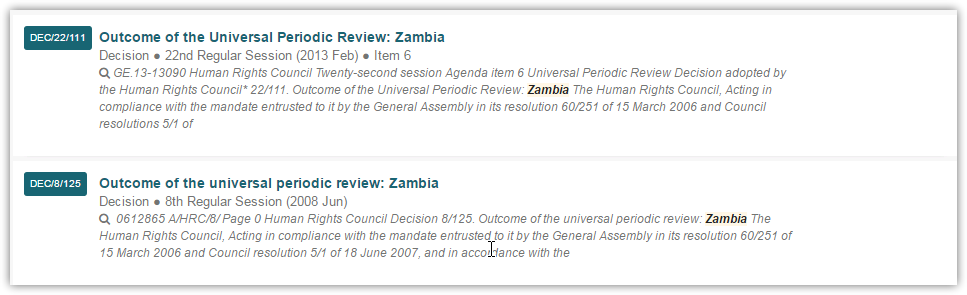
\includegraphics[width=\textwidth]{images/2016-07-15-RightDocs}
I moved to the RightDocs\index{RightDocs} website and performed a similar search. In the results list, the term I searched for is highlighted and bolded, making it really obvious where my search term shows up in the description, item name, or other metadata. I played with a few terms and found that when I search for multiple keywords, however, the results are not highlighted. I also tried to use the boolean ``AND" operator and it didn't seem to understand what my request was, resulting in different results for ``reproductive rights" and ``reproductive AND rights." So, because of this limitation, I'm not sure how it handles highlighting multiple keywords because I couldn't find an instance where two terms could be searched and displayed when they aren't right next to each other.

Also like the inroads\index{inroads} site, RightDocs\index{RightDocs} displays the currently selected search facets with the search terms together, explaining their relationship (shown below). I think that like the inroads site, I need to implement something like this for the Legal Storehouse that indicates to the user that their search terms are combined with the facets. While there isn't any indication of which facet is on an item, the ``Search Mode" switch indicates with AND/OR if the terms are inclusive or exclusive. Additionally, when an item is selected, the ``Topic" indicator in the left panel lists which categories the item has been tagged.

\begin{center}
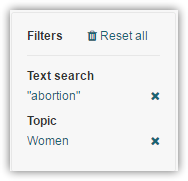
\includegraphics{2016-07-15-RightDocs-facets}
\end{center} 

\section{July 18, 2016}
Today I plan to finalize the mockup, catalog some more entries, and meet with Katrina\index{Lee, Katrina} later on in the day to begin creating a template in SiteCore.\index{SiteCore} Even though this is technically a library work day, there's a lot I'm going to need to do to prepare for meeting and update this notes document.

\subsection{Catalog issues}
It looks like the upgrade to InMagic\index{InMagic} over the weekend didn't go as smoothly as planned. The catalog is currently inaccessible and the library has been advised by IT to avoid editing or saving things in the catalog as it will most likely not be retained. This puts me back a bit because I wanted to finish working through cataloging the resources. I'll have to wait until the afternoon for IT to meet with the InMagic\index{InMagic} support team to resolve the issue.

\subsection{Meeting with Katrina}
I met with Katrina\index{Lee, Katrina} over Skype for Business to catch up on the project. Overall, she's pleased with the progress and recommended\dots

\begin{itemize}
\itemsep0em 
    \item Before we move on to creating page templates in SiteCore\index{SiteCore}, Katrina\index{Lee, Katrina} recommends that I begin thinking about what types of fields and groups of fields we will be using. To do this, she recommends that I create a spreadsheet and work through the different fields on the mockup document. From there, we can translate the spreadsheet items with actual SiteCore stuff. I need to do this in the next week. The information is located on Sheet 2 of the Legal Storehouse spreadsheet document.
    \item Create brief meta descriptions for each entry. This is different than the blurbs or abstracts and should be a summary of the document and a maximum of two lines of text. For this, Katrina\index{Lee, Katrina} explains, take the example of the text under search results on Google. \\
    \noindent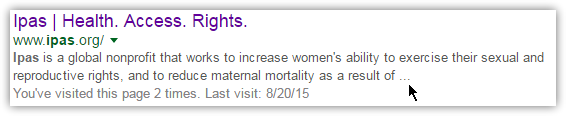
\includegraphics[width=.80\textwidth]{2016-07-18-Google}
    \item Continue cataloging all of the entries that are missing from the library catalog. This isn't necessarily a time-sensitive task, but it would be nice to have it finished.
\end{itemize}

Additionally, and most importantly, Katrina\index{Lee, Katrina} encouraged me to set up a brief check-in meeting with Patty\index{Skuster, Patty}. In that meeting, we should discuss how the current layout works, what her thoughts are on the current organization of the mockup, what the meta descriptions should be (at the time of the meeting, she expects that each item will have a meta description), and if there's any other part that Patty would like to see done differently. Additionally, I think it would be a good time to present her a working draft of this document. 

\subsection{Email to Patty}
Before the end of the day, I sent Patty\index{Skuster, Patty} another brief email requesting that we meet to touch base about the project. I also CC'd Katrina\index{Lee, Katrina} to keep her in the loop.

\vspace{2em}
\noindent
\includegraphics[height=\fontcharht\font`\B]{icons/attachment-email} See Attachment \ref{fig:2016-07-18-Email-Tim-Patty}.
\vspace{2em}

\section{July 21, 2016}
\subsection{Meeting invite}
I had a regular bi-weekly meeting with Julia\index{Cleaver, Julia} and she recommended that I invite Patty\index{Skuster, Patty} to a meeting via Outlook. If it doesn't work with her busy schedule, she could just decline the meeting invite and just propose another that works for her. I checked in with Katrina\index{Lee, Katrina} and sent Patty and Katrina a meeting invite before the end of the day.

\vspace{2em}
\noindent
\includegraphics[height=\fontcharht\font`\B]{icons/attachment-message} For the Skype for Business message, see Attachment \ref{fig:2016-07-21-Conversation-Katrina}.
\vspace{2em}

\vspace{2em}
\noindent
\includegraphics[height=\fontcharht\font`\B]{icons/attachment-calendar} For the meeting invite, see Attachment \ref{fig:2016-07-21-Meeting-invite}.
\vspace{2em}


\section{July 22, 2016}
\subsection{Meeting with Patty cancelled, email instead}
Patty\index{Skuster, Patty} said she was just about to go on vacation and recommended that I instead send her an email summary of all of the updates. I responded and indicated that I will send her questions and this document for her to look at over the weekend.

\vspace{2em}
\noindent
\includegraphics[height=\fontcharht\font`\B]{icons/attachment-email} See Attachment \ref{fig:2016-07-22-Email-Patty-Tim}.
\vspace{2em}

\subsection{Field Experience evaluation paperwork}
Lori Haight\index{Haight, Lori} emailed me needing Katrina's\index{Lee, Katrina} email address for the Field Experience evaluation paperwork due by July 28. I forwarded the paperwork to Katrina and I talked to her during the day about it. She will get it back to me and I will send it to Lori.

\vspace{2em}
\noindent
\includegraphics[height=\fontcharht\font`\B]{icons/attachment-email} See Attachment \ref{fig:2016-07-22-Email-Lori-Tim}.
\vspace{2em}

\section{July 25, 2016}
\subsection{Meeting with Katrina cancelled}
Katrina\index{Lee, Katrina} came by my desk and suggested that we meet tomorrow for our SiteCore\index{SiteCore} introduction meeting.

\section{July 26, 2016}\label{2016-07-26}
\subsection{Meeting with Katrina}
Katrina\index{Lee, Katrina} and I met today and started creating a metadata template in SiteCore\index{SiteCore} using entries from the second page of the Legal Storehouse page. It took some time to understand the relationship between fields for controlled vocabulary and tree-ed information, but we figured it out after playing with it. We created about 10 unique fields, with about 20 fields total. By the end of the meeting, we were pretty pleased with our template and I think I'm ready to start working to move the entries from the spreadsheet over into SiteCore\index{SiteCore}. 

All that I'm waiting on now is a login to SiteCore\index{SiteCore} from Kyle\index{Goetschius, Kyle} and I can start creating the items with the metadata template.

\vspace{2em}
\noindent
\includegraphics[height=\fontcharht\font`\B]{icons/attachment-email} See Attachment \ref{fig:2016-07-26-Email-Katrina-Kyle-Tim}.
\vspace{2em}

\section{July 28, 2016}
\subsection{Field Experience evaluation paperwork completed}
Katrina\index{Lee, Katrina} filled out the paperwork last night and I signed off on it. I scanned it and plan to attach it to an email to Lori\index{Haight, Lori}. I also plan to send it to Melanie\index{Feinberg, Melanie} today along with this document. 

\vspace{2em}
\noindent
\includegraphics[height=\fontcharht\font`\B]{icons/attachment-email} See Attachment \ref{fig:2016-07-28-Evaluation-Site-Supervisor}.
\vspace{2em}

\section{July 29, 2016}
\subsection{Reminder email sent about SiteCore access}
I sent an email reply to Katrina's previous update message (see Attachment \ref{fig:2016-07-29-Email-Katrina-Kyle-Tim}) requesting an update from Kyle\index{Goetschius, Kyle} about the current progress for getting a login for SiteCore\index{SiteCore}. Katrina\index{Lee, Katrina} was CC'd on the message. I did not receive a response.

\vspace{2em}
\noindent
\includegraphics[height=\fontcharht\font`\B]{icons/attachment-email} See Attachment \ref{fig:2016-07-29-Email-Tim-Kyle-Katrina}.
\vspace{2em}

\section{August 2, 2016}\label{2016-08-02}
\subsection{Skype for Business message from Katrina}
This morning, Katrina\index{Lee, Katrina} sent me a message and explained that her mother would be undergoing surgery on the day we had planned to meet with Dr. Feinberg\index{Feinberg, Melanie} via Skype. She requested that we move the date for the call to another day. I emailed Dr. Feinberg and requested some dates. 

\vspace{2em}
\noindent
\includegraphics[height=\fontcharht\font`\B]{icons/attachment-message} For the message from Katrina, see Attachment \ref{fig:2016-08-02-Message-Katrina-Tim}.
\vspace{2em}

\vspace{2em}
\noindent
\includegraphics[height=\fontcharht\font`\B]{icons/attachment-email} For the complete email correspondence about the logistics of the meeting reschedule, see Attachment \ref{fig:2016-08-03-Email-Tim-Melanie}.
\vspace{2em}

\subsection{Email to Lori Haight}
I emailed Lori\index{Haight, Lori} to update her on the progress of my work in the Field Experience and to explain why I had missed the deadline. She responded soon after and assured me that as soon as the paperwork reaches her desk, she will amend the ``I'' or ``Incomplete'' grade that has been entered in ConnectCarolina\index{ConnectCarolina}.

\vspace{2em}
\noindent
\includegraphics[height=\fontcharht\font`\B]{icons/attachment-email} See Attachment \ref{fig:2016-08-02-Email-Tim-Lori}.
\vspace{2em}

\section{August 3, 2016}\label{2016-08-03}
\subsection{Skype call with Katrina and Dr. Feinberg}
After a few schedule changes, we decided to meet this morning over Skype. Katrina\index{Lee, Katrina}, Dr. Feinberg\index{Feinberg, Melanie}, and I talked about the most recent changes to the project and discussed some of the UNC requirements for the Field Experience grade. As of July 28th, Lori\index{Haight, Lori} has inputted an ``I'' or ``Incomplete'' for the course grade for this semester. I relayed that to Dr. Feinberg and assured her that the work will continue to progress on the site. I suggested that the project will be completed by Thanksgiving.

In the meantime, I will continue working on the site and I will also be writing the reflection paper assignment that is required for SILS. Dr. Feinberg said that she would send me a few articles that she recommends. Namely, they will discuss the differences in recall techniques for medical and legal documents. She noted that in many cases, the practices overlap, but they mostly assume that the intended audience is made up of lawyers or doctors---professional practitioners. Since the Legal Storehouse site is mostly intended for policy and grant writers (e.g. non-specialized practitioners), the articles may not completely apply to my situation. Dr. Feinberg recommended that Katrina\index{Lee, Katrina} and I talk with Patty\index{Skuster, Patty} to double check what types of users she anticipates will visit the site. In most cases, we expect it will be people who are already knowledgeable about the document creators (e.g. WHO, names of specific authors, Ipas, etc.) and not much explanation will be needed to justify why these sources were included in the list. To this point, Dr. Feinberg noted that she may be able to find some recommended resources for the topic, but may be hard pressed to find anything. In any case, she will send me the ``canonical'' articles that discus information and document recall to help me get started. I also explained that for most of the reflection paper, I will be recapping this document and explaining my work log in greater detail.

% Primarily, the meeting consisted of me explaining to Dr. Feinberg\index{Feinberg, Melanie} why the project has moved slowly while trying my best to make sure I didn't throw Katrina\index{Lee, Katrina} under the bus. There was no way I was going to make her or anyone else at Ipas look bad with her sitting at the meeting, but the fact remains that my work has been severely delayed by their ineptitude in managing an Outlook inbox, their inability to complete simple tasks, and their incalculable absences from the office. I am embarrassed to report to Dr. Feinberg---someone with whom I had hoped to ask to supervise my Master's thesis---that up until this meeting, I had done no concrete work on the Legal Storehouse website. I was put in the awkward situation where I must explain the situation of which I am fully responsible to my faculty supervisor in a way that doesn't offend my work supervisor---the one who is fully to blame for the ``Incomplete'' I received on my academic record. After this meeting, I do not expect that Dr. Feinberg will be inclined to agree to supervise my master's work. At the end of the day, I have wasted my entire summer by registering and paying over \$3,000 for a Field Experience, performing over 100 hours of busy work, sending countless unanswered emails and meeting requests, and covering for everyone at Ipas when they drop the ball.

Dr. Feinberg noted that although I didn't include it in my Field Experience proposal or in my Learning Objectives in the Agreement document, the comparative assessment has taken most of my time for the project. She noted that this was important to understand that in many situations when working on professional projects, the things that take the most time are often unanticipated. She noted that it was important to include information abotu this and about the work itself when it comes to the Comparative Analysis because it can help me plan more effectively in the future. We finished the call and I ensured her that I will stay in contact with her about the work throughout the fall semester.

\vspace{2em}
\noindent
\includegraphics[height=\fontcharht\font`\B]{icons/attachment-email} For information about logistics for the Skype call, see Attachments \ref{fig:2016-08-03-Email-Tim-Melanie} and \ref{fig:2016-08-03-Email-Tim-Katrina}.
\vspace{2em}

\section{August 8, 2016}\label{2016-08-08}
\subsection{Check-in meeting with Katrina}
Katrina\index{Lee, Katrina} and I had a quick check-in meeting to discuss creating the analytics plan and the maintenance plan. I had sent her a message earlier in the week requesting some guidance on how to begin writing the maintenance plan and the analytics plan---a task that we had listed as one of my learning objectives for the Field Experience. She wanted to wait to discuss the plans at our meeting for today (August 8th).

\vspace{2em}
\noindent
\includegraphics[height=\fontcharht\font`\B]{icons/attachment-message} For the Skype message from me to Katrina, see Attachment \ref{fig:2016-08-02-Message-Tim-Katrina}.
\vspace{2em}

\subsubsection{Maintenance plan}
For the maintenance plan, Katrina recommended that I sit down with Patty\index{Skuster, Patty} and the communications department to outline when and how the site will be updated. She stressed that I will have to balance the need to keep the site up to date and the amount of time that the Communications department expects to be able to spend on the task. Aside from adding or deleting content when replacements become available, the very least we need to do is to ensure that all of the links to external sites are accessible and continue to resolve after the site becomes live. I noted that the documents will all be in the Ipas Library catalog, but since the catalog isn't open to the public, this won't be of much use to visitors to the site. Katrina noted that SiteCore\index{SiteCore} has a link checker as a built-in function, so she or someone in Communications will most likely be the point person for checking that the links work and updating them if they are unavailable. Katrina noted that I have to write in the Maintenance Plan specific details for how to update the site, but most importantly, \ul{who} will update the site. It's not terribly important which department at Ipas is responsible for the task, but it's crucial to see which individual person will take ownership. Without that responsibility, it will fall into the cracks and never get done.

For the Legal Storehouse, Katrina recommended that I write the Maintenance Plan document with the guideline that the site will need to be audited at least twice a year. This will ensure that the links will be accessible and that the documents are up to date. Additionally, the maintenance plan will need to allude to the analytics plan---both will influence each other.

\subsubsection{Analytics plan}
This plan will be a bit more difficult, Katrina noted, because there is no way to anticipate what kind of analytics information we'll receive from SiteCore\index{SiteCore} once the site goes live. In a year, we will understand how people use the site, but as of now, we can't really make recommendations for changes if we have no way of knowing what is lacking and what features, facets, or documents are the most popular. There are some general principles to actionable analytics, but there's nothing solid that I can put down in a document that explains what steps to take in response to the analytics. 

In any case, the Communications unit will receive the analytics information on a regular basis and the actionable data is easily accessible. In the future, we just need to request the Coveo\index{Coveo} data from the Comms. unit and we should have what we're looking for. She recommended that we meet once a year to discuss the results and to make decisions on how to move forward. In many cases, the analytics will give us information on searched terms, but she's also interested in identifying where possible UX bottlenecks arise (e.g. when it's too difficult to find the download link) and propose changes to the site structure to better fit the audience. She wasn't completely sure what types of information Coveo will provide, but she is sure that there is at least some ability to link analytical information with user behavior. We will use this functionality to make sure that the site continues to be useful to visitors.

Katrina also noted that since the site is using a ``bucket'' structure to display information, it will be more difficult to understand usage data compared to other pages on the Ipas website. On most other sites, page views and navigation between pages generates actionable metrics that can be used to understand how the site is being used. Since the main functionality of the site is just a list of results, we'll have to think differently about how to track what people are accessing. To do this, Katrina expects that Coveo\index{Coveo} has some built-in capabilities that, in addition to tracking search terms, allow us to track facet use, which sections were expanded (in this case, we're interested in seeing who accessed the ``read more'' section), and which external links are associated with facet and search term pairs. Additionally, since the user will just be on one page, it will be easier to track total time on the site, giving us more information about how long it takes for someone to find what they're looking for. All of this will help us understand our users better and as long as we figure out what Coveo is able to do, we should be on track to understanding for what purpose people are using the site, and to identify where we need to make changes to improve site navigation and document recall.

\subsection{Email from Patty}
Patty\index{Skuster, Patty} sent me an email earlier in the day and explained that she was back from vacation and was interested in meeting to talk about the Legal Storehouse work. I sent her and Katrina an event invite to meet on August 10th. Patty accepted the event and Katrina tentatively accepted. I'm not sure what Patty would like to talk about, but per my previous email, I expect that I will be catching her up on the spreadsheet work and getting some feedback about users, the mockup, and whether or not I'm working in the direction that she was anticipating when we spoke a few months ago. 

\vspace{2em}
\noindent
\includegraphics[height=\fontcharht\font`\B]{icons/attachment-email} For Patty's email, see Attachment \ref{fig:2016-08-08-Email-Patty-Tim}.
\vspace{2em}

\vspace{2em}
\noindent
\includegraphics[height=\fontcharht\font`\B]{icons/attachment-calendar} For the meeting invite, see Attachment \ref{fig:2016-08-08-Meeting-Tim-Patty-Katrina}.
\vspace{2em}

% \section{August 9, 2016}
% \subsection{Quick conversation with Julia about SiteCore}
% Julia\index{Cleaver, Julia} has returned from her summer vacation and talked to me in the morning. She was frustrated that Kyle\index{Goetschius, Kyle} still has not created a login for me on SiteCore\index{SiteCore}. I agreed with her and summarized my meeting between Dr. Feinberg\index{Feinberg, Melanie} and Katrina\index{Lee, Katrina}. I explained that Thanksgiving was my new deadline and that I would remain working on cataloging the remaining Legal Storehouse documents.

\section{August 10, 2016}
\subsection{Email }
\subsection{Skype meeting with Patty and Katrina}
In the afternoon, I met with Patty\index{Skuster, Patty} and Katrina\index{Lee, Katrina} over Skype for Business to talk about some of the updates to the Legal Storehouse. Patty was pleased with the progress and is excited to see the project continuing. In response to my email sent FIXME\todo{Double check this date}, Patty had a few updates to the questions that I had and cleared up some of the questions that I had. She also had some comments. Namely\dots
\begin{itemize}
    \item The article from FIGO needs to be the task force report. She needs an updated PDF and citation for that resource.
    \item There are a few entries from the Anand Grover and UN Rapporteurs that need to be split up into several entries. There are a few specific ones that she highlighted in the spreadsheet.
    \item Patty will go into the spreadsheet and update some of the metadescriptions that I wasn't able to get. She has some legal-specific comments that she wants to explain as an abstract-like blurb.
\end{itemize}

\clearpage
\section*{List of Attachments}

\begin{sidewaysfigure}[ht]
   \centering
        \noindent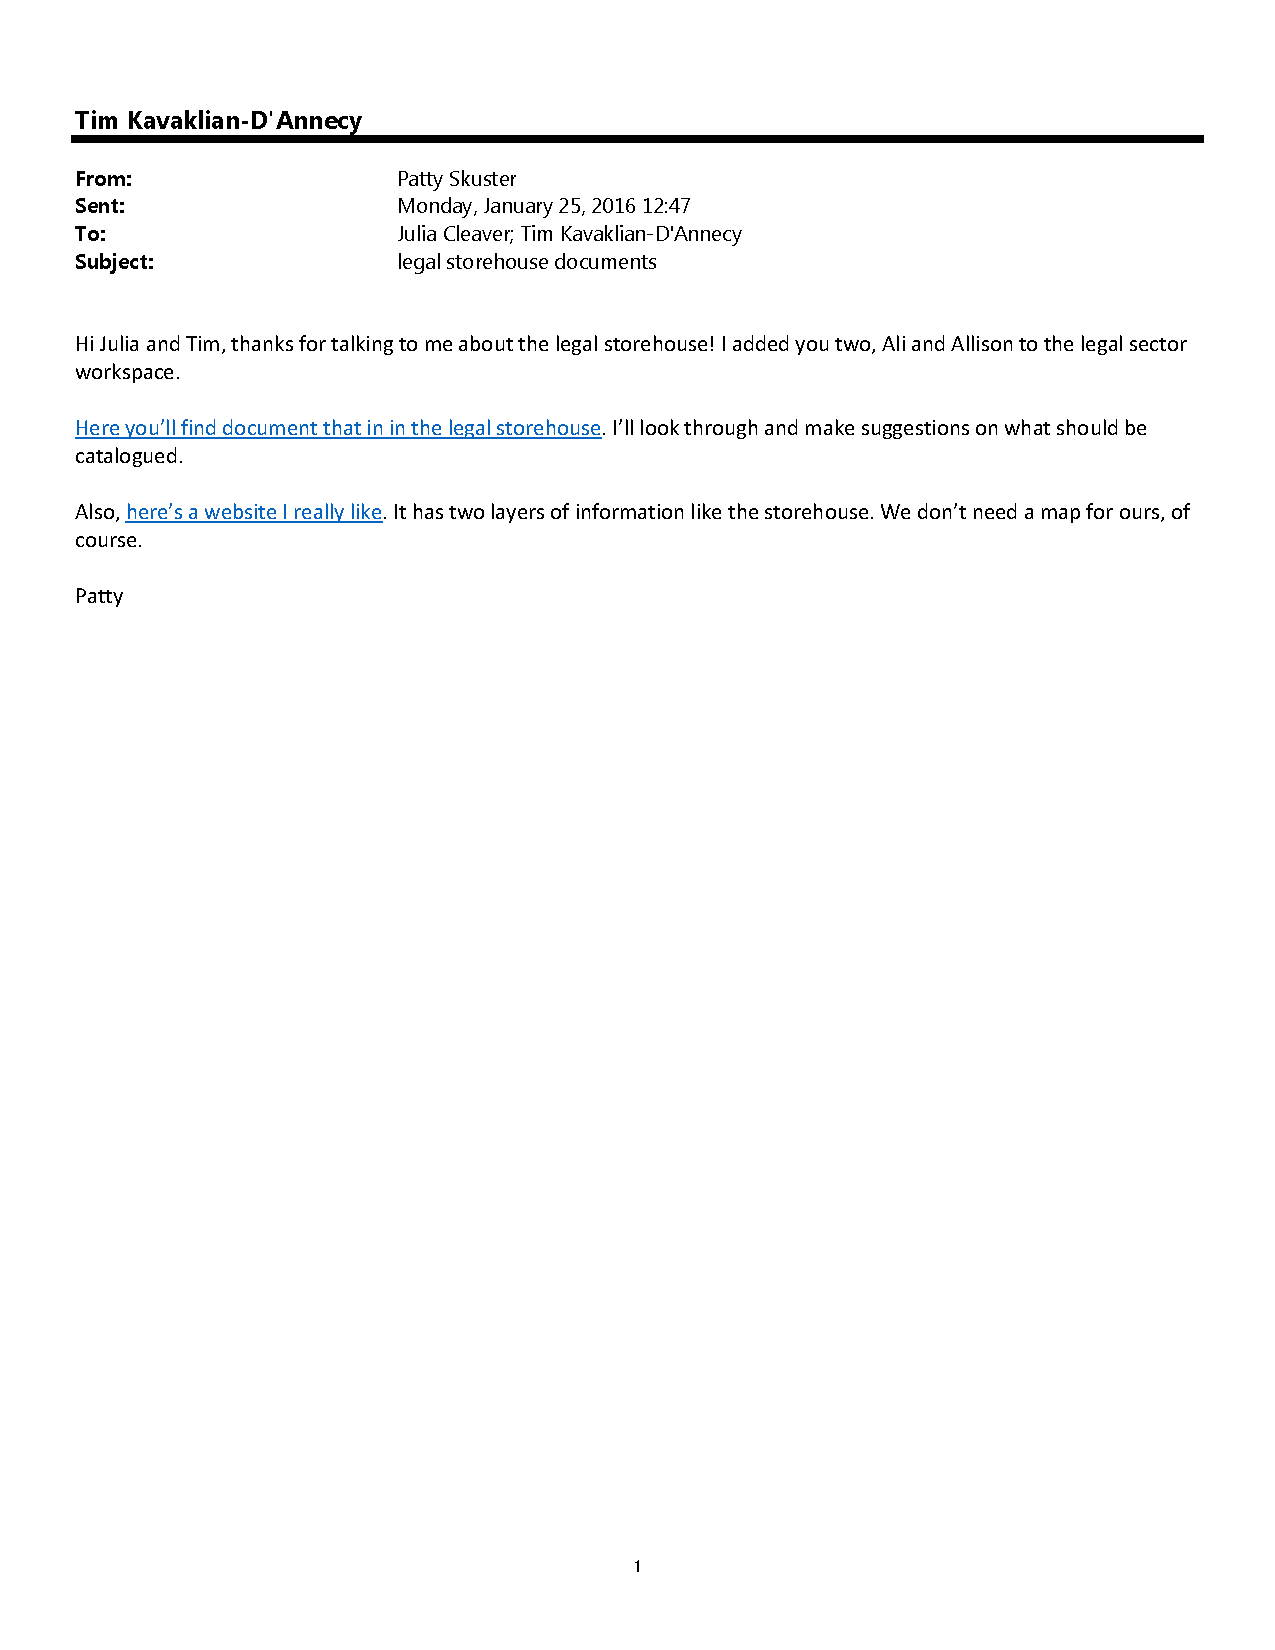
\includegraphics[page=1,angle=-90,origin=c,width=.75\textwidth,height=.75\textheight]{documents/2016-01-25-Email-Patty.pdf} \hfill 
 \caption{Email dated January 25, 2016 from Patty\index{Skuster, Patty} to Tim and Julia\index{Cleaver, Julia} introducing the Legal Storehouse.}
 \label{fig:2016-01-25-Email-Patty}
\end{sidewaysfigure}

\begin{sidewaysfigure}[ht]
   \centering
       \noindent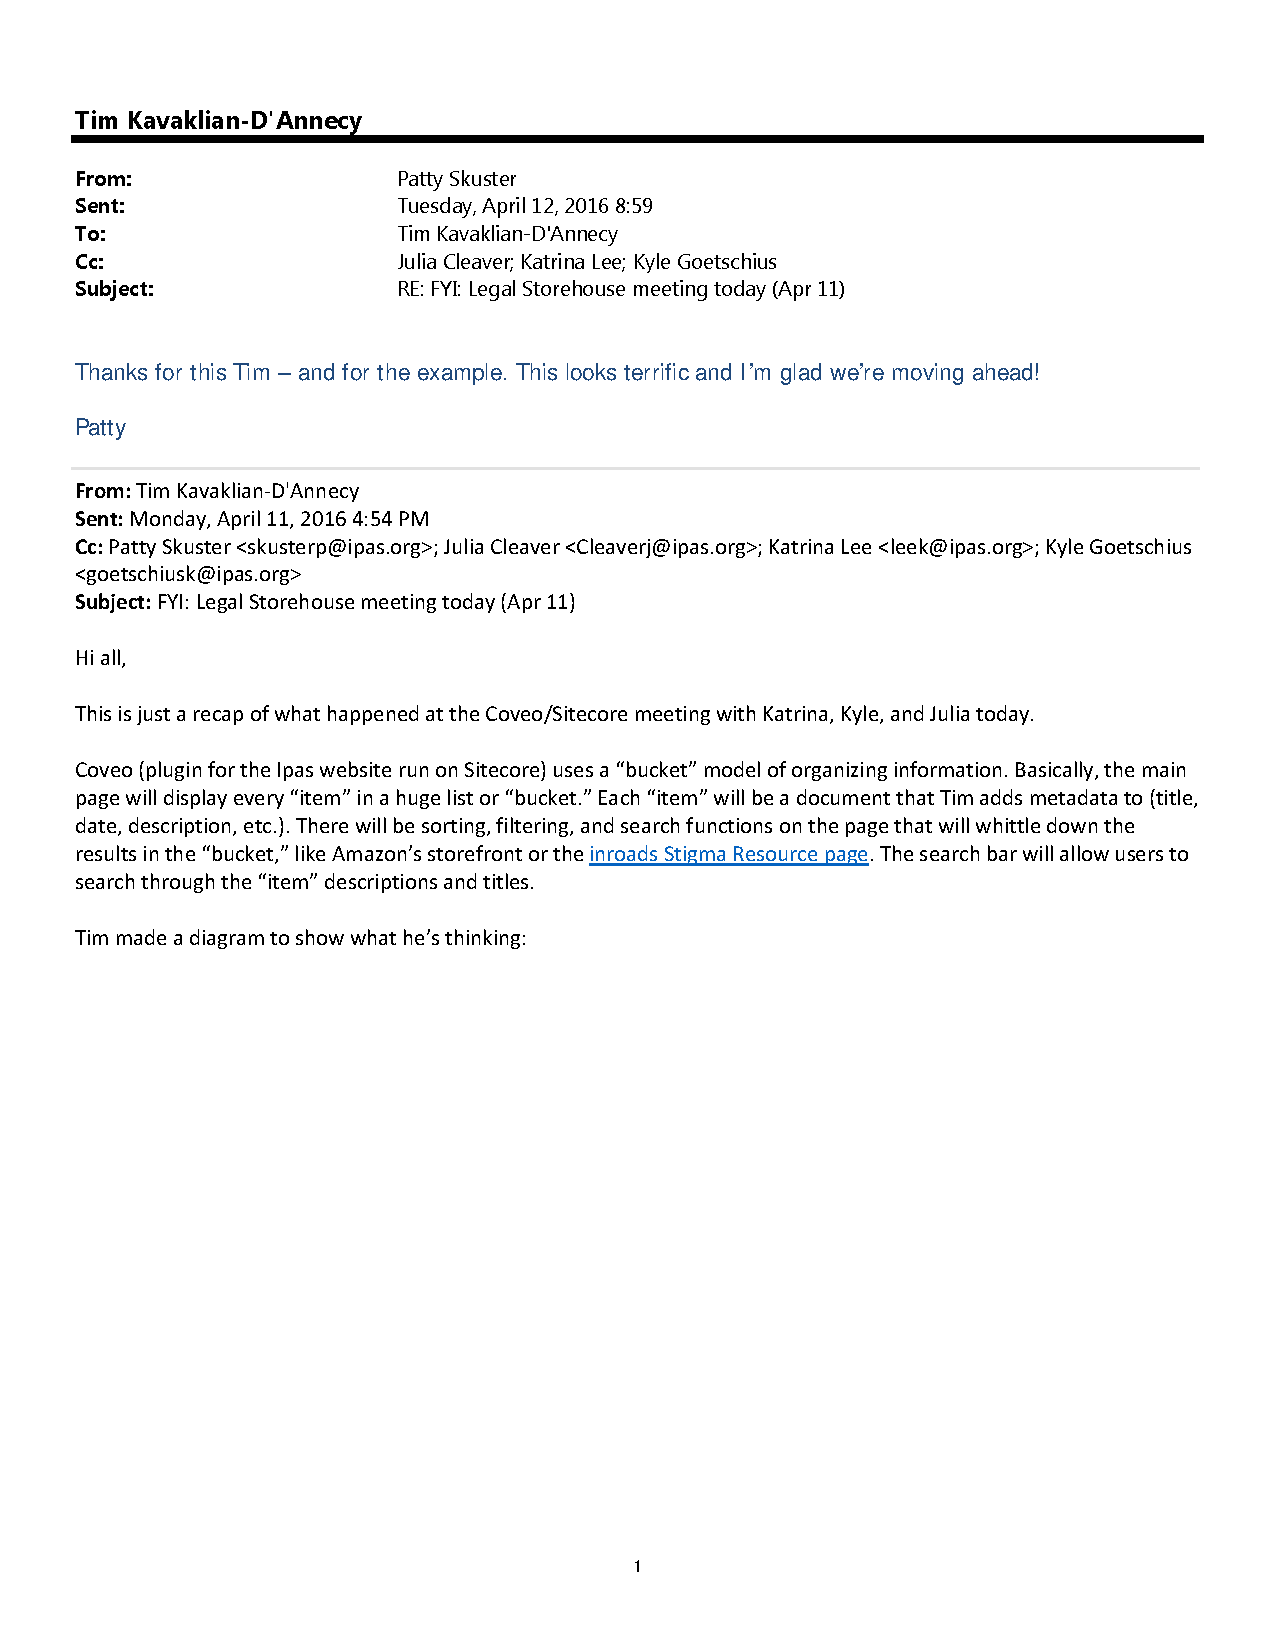
\includegraphics[page=1,width=.45\textwidth]{documents/2016-04-11-Email-Tim.pdf} \hfill 
       \noindent\includegraphics[page=2,width=.45\textwidth]{documents/2016-04-11-Email-Tim.pdf}
 \caption{Email dated April 11, 2016 from Tim to several people in Ipas recapping the meeting that took place today. See section~\protect\ref{2016-04-11} for information about that meeting.}
 \label{fig:2016-04-11-Email-Tim}
\end{sidewaysfigure}

\begin{sidewaysfigure}[ht]
   \centering
        \noindent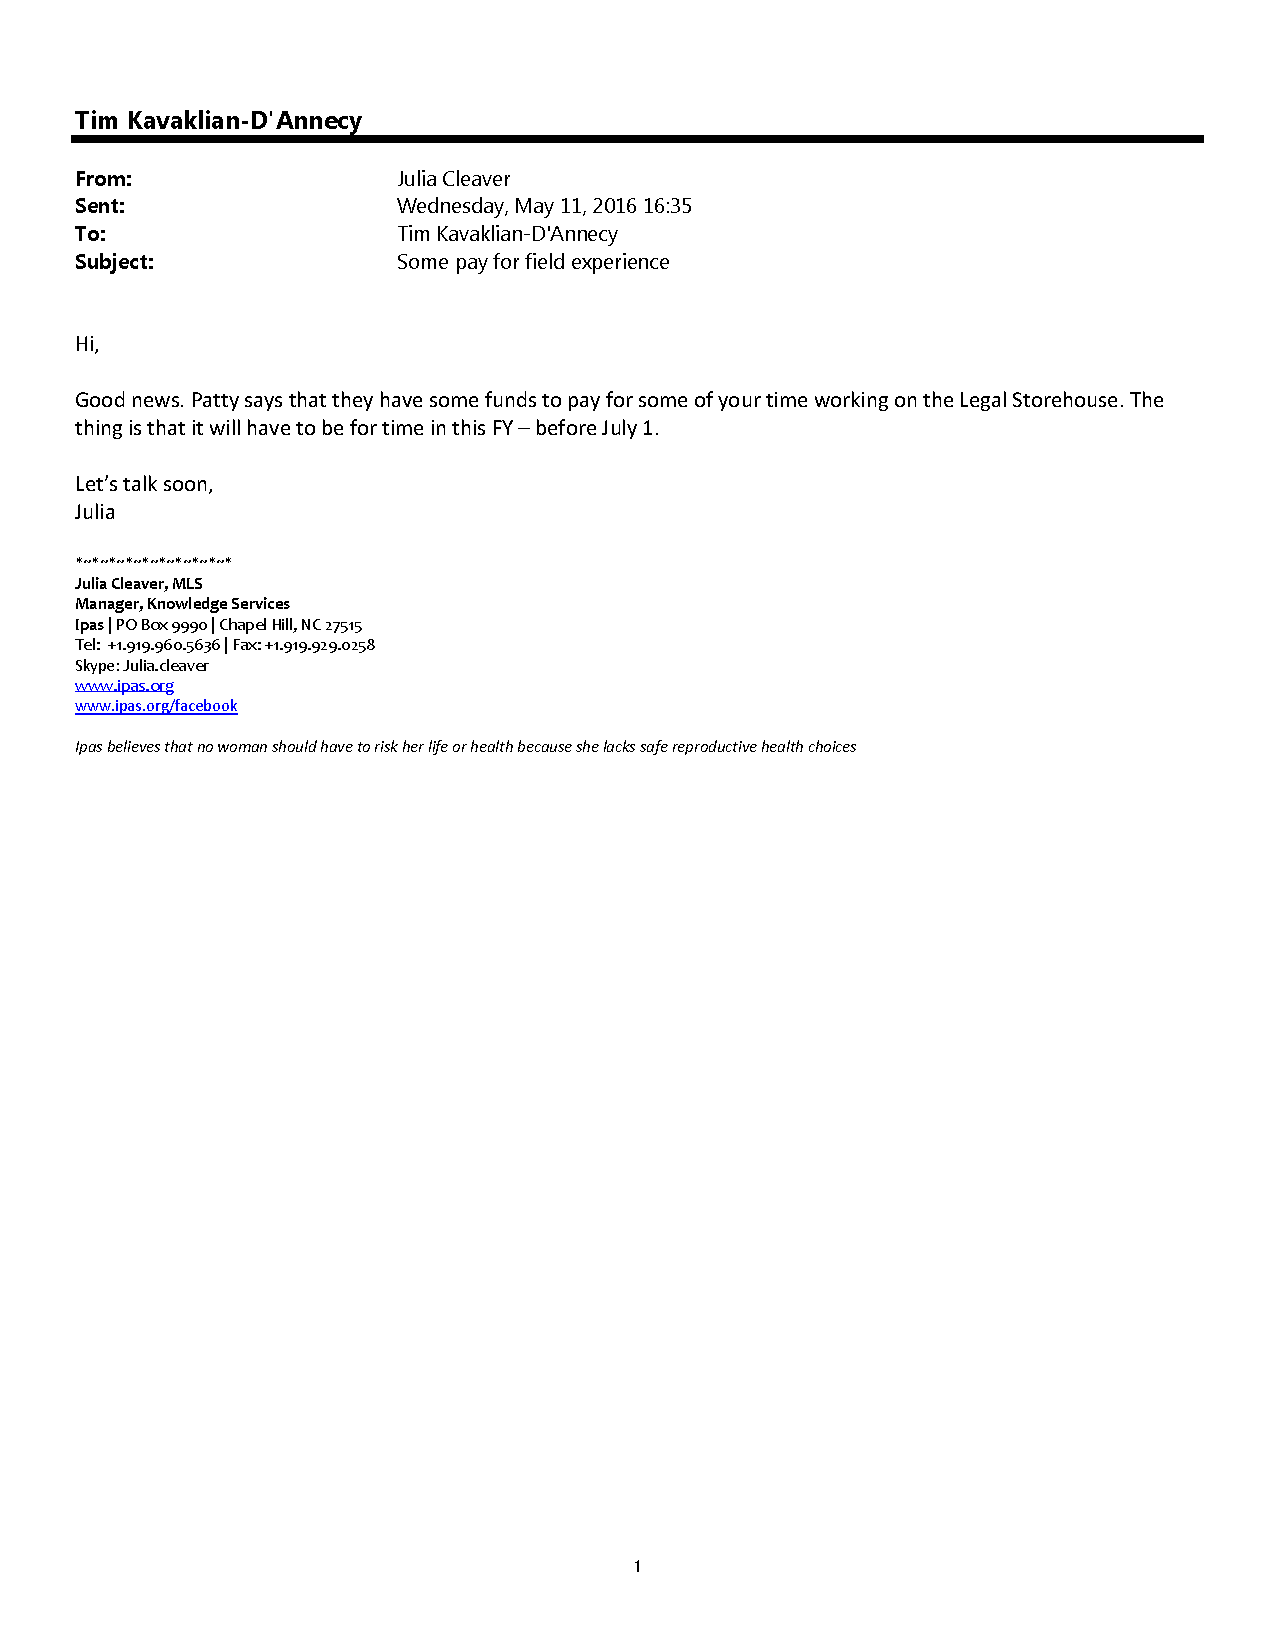
\includegraphics[page=1,angle=-90,origin=c,width=.75\textwidth,height=.75\textheight]{documents/2016-05-11-Email-Julia-Cleaver.pdf}
 \caption{Email dated May 11, 2016 from Julia Cleaver\index{Cleaver, Julia} discussing Ipas pay for the Field Experience.}
 \label{fig:2016-05-11-Email-Julia-Cleaver}
\end{sidewaysfigure}

\begin{sidewaysfigure}[ht]
   \centering
       \noindent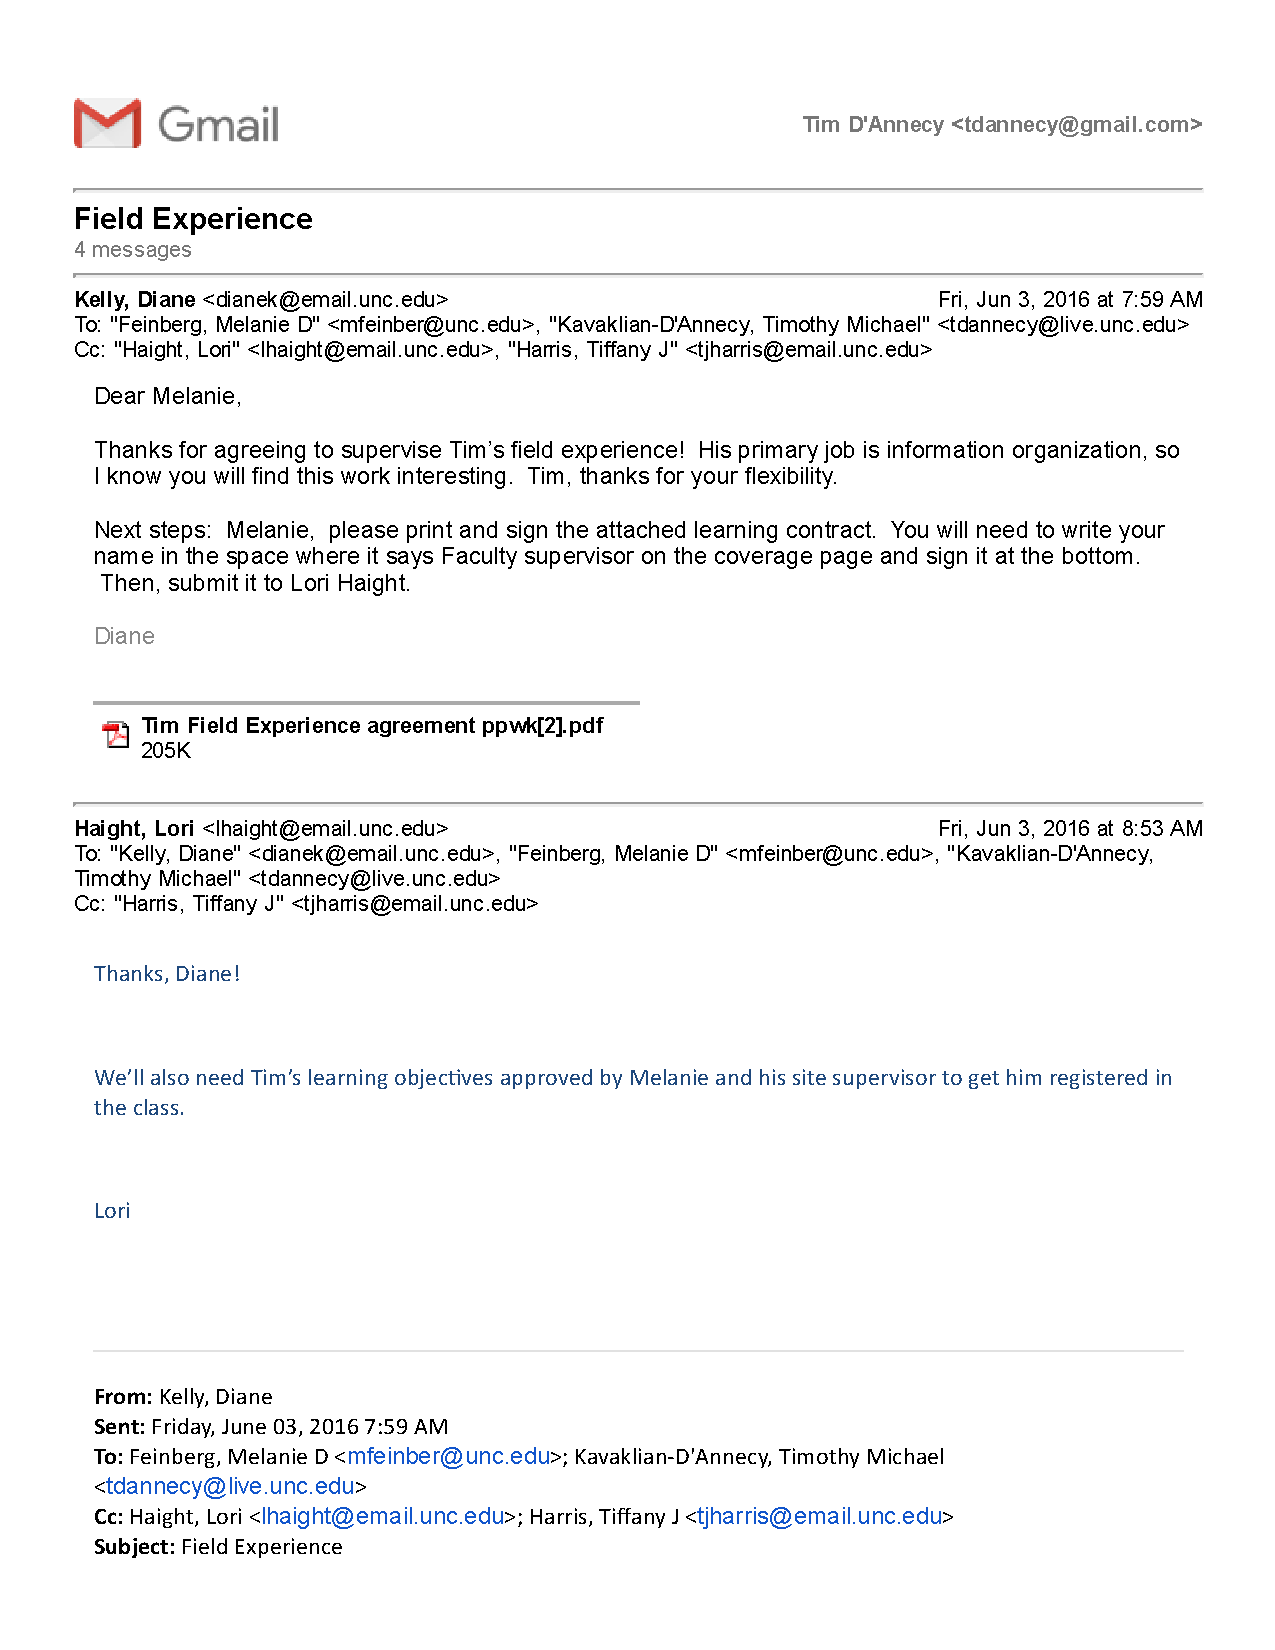
\includegraphics[page=1,width=.45\textwidth]{documents/2016-06-03-Email-Diane-Kelly.pdf} \hfill 
       \noindent\includegraphics[page=2,width=.45\textwidth]{documents/2016-06-03-Email-Diane-Kelly.pdf}
 \caption{Email dated June 3, 2016 from Diane Kelly to several recipients at UNC noting that Melanie Feinberg\index{Feinberg, Melanie|textbf} to be Tim's Faculty Supervisor for the Field Experience.}
 \label{fig:2016-06-03-Email-Diane-Kelly}
\end{sidewaysfigure}

\begin{sidewaysfigure}[ht]
   \centering
       \noindent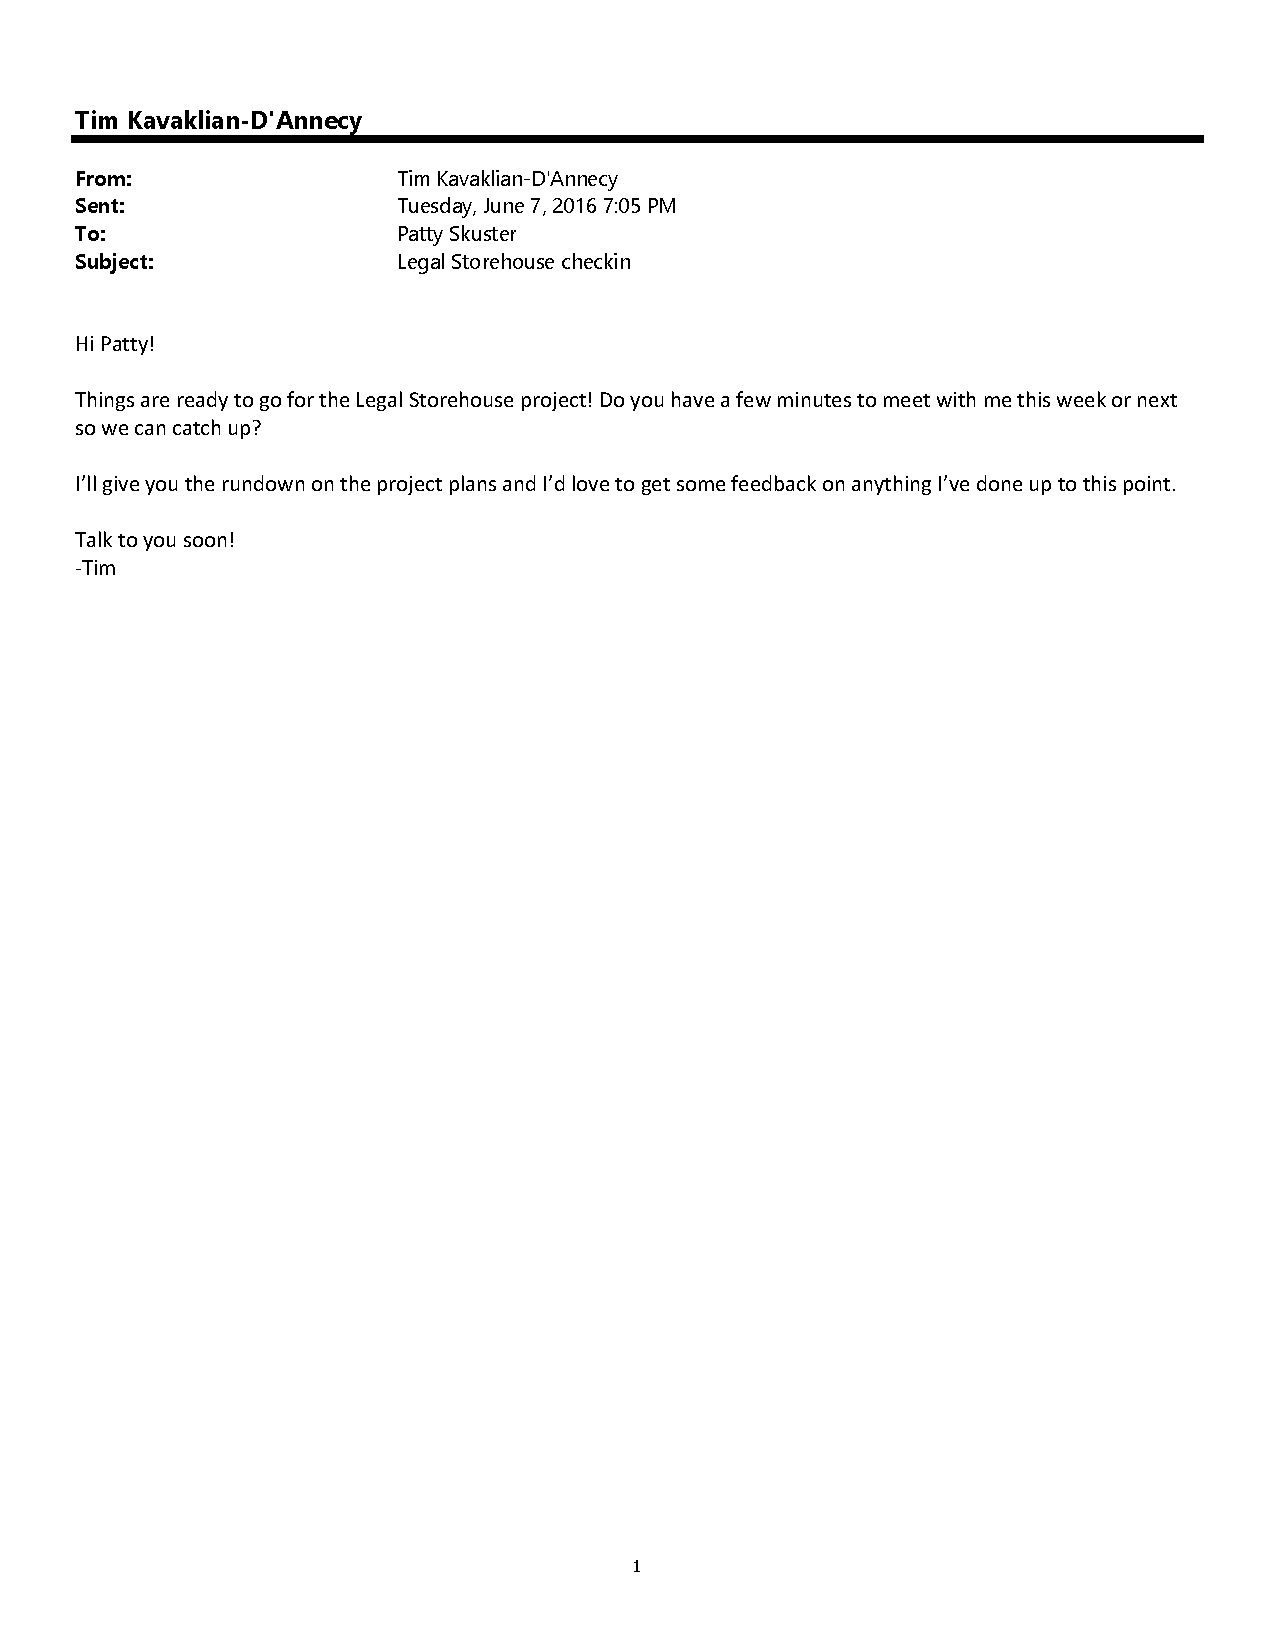
\includegraphics[page=1,angle=-90,origin=c,width=.75\textwidth,height=.75\textheight]{documents/2016-06-07-Email-Tim-Patty.pdf}
 \caption{Email dated June 7, 2016 from Tim to Patty\index{Skuster, Patty} asking to set up a quick meeting.}
 \label{fig:2016-06-07-Email-Tim-Patty}
\end{sidewaysfigure}

\begin{sidewaysfigure}[ht]
   \centering
       \noindent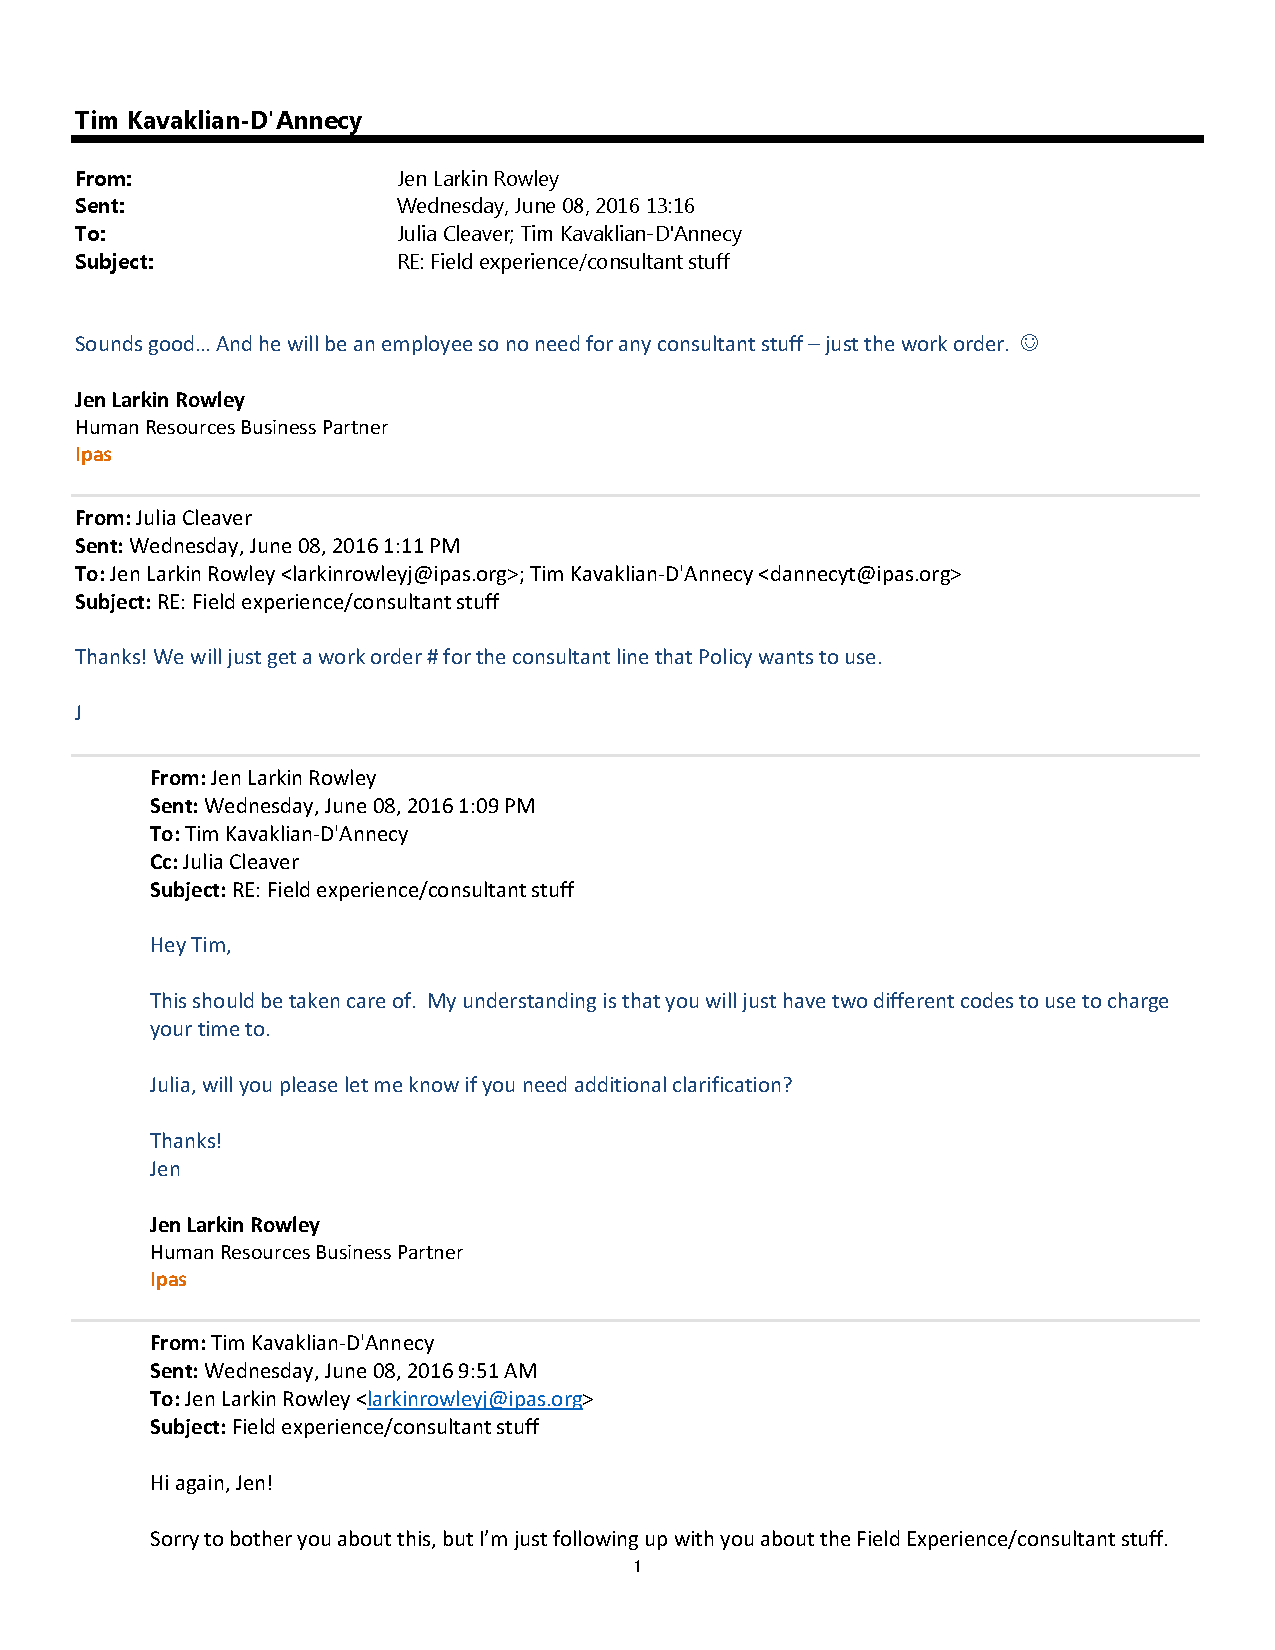
\includegraphics[page=1,width=.45\textwidth]{documents/2016-06-08-Email-Jen-Larkin.pdf} \hfill 
       \noindent\includegraphics[page=2,width=.45\textwidth]{documents/2016-06-08-Email-Jen-Larkin.pdf}
 \caption{Email dated June 8, 2016 from Tim to Jen Larkin\index{Larkin Rowley, Jen} about updates for pay. Responses included from Julia\index{Cleaver, Julia}.}
 \label{fig:2016-06-08-Email-Jen-Larkin}
\end{sidewaysfigure}

\begin{sidewaysfigure}[ht]
   \centering
       \noindent\includegraphics[page=1,angle=-90,origin=c,width=.75\textwidth,height=.75\textheight]{documents/2016-06-13-Email-Patty.pdf}
 \caption{Email dated June 13, 2016 from Patty\index{Skuster, Patty} to Tim with new work order number for Policy.}
 \label{fig:2016-06-13-Email-Patty}
\end{sidewaysfigure}

\begin{sidewaysfigure}[ht]
   \centering
       \noindent\includegraphics[page=1,width=.45\textwidth]{documents/2016-06-13-Email-Julia} \hfill 
       \noindent\includegraphics[page=2,width=.45\textwidth]{documents/2016-06-13-Email-Julia} 
 \caption{Email dated June 13, 2016 between Julia\index{Cleaver, Julia} and Tim talking with HR about issues with reporting time sheets on Vega\index{Vega}.}
 \label{fig:2016-06-13-Email-Julia}
\end{sidewaysfigure}
\clearpage
\begin{sidewaysfigure}
\centering
   \noindent\includegraphics[page=3,angle=-90,origin=c,width=.75\textwidth,height=.75\textheight]{documents/2016-06-13-Email-Julia}
\end{sidewaysfigure}


\begin{sidewaysfigure}[ht]
   \centering
       \noindent\includegraphics[page=1,width=\textwidth]{documents/2016-06-28-spreadsheet} \hfill 
        \caption{Legal Storehouse spreadsheet, as of June 28, 2016.}
 \label{fig:2016-06-28-spreadsheet}
\end{sidewaysfigure}
\clearpage
\begin{sidewaysfigure}[ht]
\centering
       \noindent\includegraphics[page=1,width=\textwidth]{{documents/2016-06-28-spreadsheet}} \hfill
\end{sidewaysfigure}

\begin{sidewaysfigure}[ht]
   \centering
      \noindent\includegraphics[width=\textwidth]{2016-07-15-mockup}\hfill
 \caption{Mockup of the Legal Storehouse as of July 15, 2016. Created with Draw.io\index{draw.io}}
 \label{fig:2016-07-15-mockup}
\end{sidewaysfigure}

\begin{sidewaysfigure}[ht]
   \centering
   \noindent\includegraphics[page=1,angle=-90,origin=c,width=.75\textwidth,height=.75\textheight]{documents/2016-07-18-Email-Tim-Patty}
 \caption{Email dated July 18, 2016 from Tim to Patty\index{Skuster, Patty} and CC'd to Katrina\index{Lee, Katrina} requesting a touch-base meeting.}
 \label{fig:2016-07-18-Email-Tim-Patty}
\end{sidewaysfigure}

\begin{sidewaysfigure}[ht]
  \centering
  \noindent\includegraphics[page=1,angle=-90,origin=c,width=.75\textwidth,height=.75\textheight]{documents/2016-07-21-Conversation-Katrina}
 \caption{Skype conversation dated July 22, 2016 between Tim and Katrina\index{Lee, Katrina} discussing sending an Outlook meeting invitation to Patty\index{Skuster, Patty}.}
 \label{fig:2016-07-21-Conversation-Katrina}
\end{sidewaysfigure}

\begin{sidewaysfigure}[ht]
  \centering
  \noindent\includegraphics[page=1,angle=-90,origin=c,width=.75\textwidth,height=.75\textheight]{documents/2016-07-21-Meeting-invite}
 \caption{Meeting invite sent July 22, 2016 from Tim to Patty\index{Skuster, Patty} and Katrina\index{Lee, Katrina}.}
 \label{fig:2016-07-21-Meeting-invite}
\end{sidewaysfigure}

\begin{sidewaysfigure}[ht]
  \centering
  \noindent\includegraphics[page=1,angle=-90,origin=c,width=.75\textwidth,height=.75\textheight]{documents/2016-07-22-Email-Patty-Tim}
 \caption{Email dated July 22, 2016 between Tim and Patty\index{Skuster, Patty} responding to the Outlook meeting invite agreeing to an email conversation in lieu of an in-person meeting.}
 \label{fig:2016-07-22-Email-Patty-Tim}
\end{sidewaysfigure}

\begin{sidewaysfigure}[ht]
   \centering
       \noindent\includegraphics[page=1,width=.45\textwidth]{documents/2016-07-22-Email-Lori-Tim} \hfill 
       \noindent\includegraphics[page=2,width=.45\textwidth]{documents/2016-07-22-Email-Lori-Tim} \hfill 
 \caption{Email dated July 22, 2016 from Lori\index{Haight, Lori} to Tim requesting Katrina's\index{Lee, Katrina} email address for the Field Experience site supervisor evaluation form due July 28, 2016.}
 \label{fig:2016-07-22-Email-Lori-Tim}
\end{sidewaysfigure}
\index{Lee, Katrina}
\clearpage
\begin{sidewaysfigure}
  \centering
    \noindent\includegraphics[page=3,width=.45\textwidth]{documents/2016-07-22-Email-Lori-Tim} \hfill
    \noindent\includegraphics[page=4,width=.45\textwidth]{documents/2016-07-22-Email-Lori-Tim}
\end{sidewaysfigure}


\begin{sidewaysfigure}[ht]
  \centering
  \noindent\includegraphics[page=1,angle=-90,origin=c,width=.75\textwidth,height=.75\textheight]{documents/2016-07-26-Email-Katrina-Kyle-Tim}
 \caption{Email dated July 26, 2016 from Katrina\index{Lee, Katrina} to Tim and Kyle\index{Goetschius, Kyle} recapping the meeting to create a template in SiteCore\index{SiteCore}. See Section \protect\ref{2016-07-26}.}
 \label{fig:2016-07-26-Email-Katrina-Kyle-Tim}
\end{sidewaysfigure}

\begin{sidewaysfigure}[ht]
   \centering
       \includegraphics[page=1,width=.45\textwidth]{documents/2016-07-28-Evaluation-Site-Supervisor} \hfill 
       \includegraphics[page=2,width=.45\textwidth]{documents/2016-07-28-Evaluation-Site-Supervisor} \hfill 
 \caption{Evaluation by Katrina per the Field Experience requirements. Dated July 28, 2016.}
 \label{fig:2016-07-28-Evaluation-Site-Supervisor}
\end{sidewaysfigure}
\index{Lee, Katrina}
\clearpage
\begin{sidewaysfigure}
  \centering
    \noindent\includegraphics[page=3,width=.45\textwidth]{documents/2016-07-28-Evaluation-Site-Supervisor}\hfill
    \noindent\includegraphics[page=4,width=.45\textwidth]{documents/2016-07-28-Evaluation-Site-Supervisor}
\end{sidewaysfigure}
\clearpage
\begin{sidewaysfigure}
  \centering
    \noindent\includegraphics[page=5,width=.45\textwidth]{documents/2016-07-28-Evaluation-Site-Supervisor} \hfill
    \noindent\includegraphics[page=6,width=.45\textwidth]{documents/2016-07-28-Evaluation-Site-Supervisor}
\end{sidewaysfigure}

\begin{sidewaysfigure}[ht]
  \centering
        \noindent\includegraphics[page=1,angle=-90,origin=c,width=.75\textwidth,height=.75\textheight]{documents/2016-07-29-Email-Tim-Kyle-Katrina}
 \caption{Email dated July 29 from Tim in response to Katrina's\index{Lee, Katrina} email at Attachment \ref{fig:2016-07-26-Email-Katrina-Kyle-Tim} requesting an update from Kyle\index{Goetschius, Kyle} about SiteCore\index{SiteCore} access.}
 \label{fig:2016-07-29-Email-Tim-Kyle-Katrina}
\end{sidewaysfigure}

fig:2016-07-29-Email-Katrina-Kyle-Tim

\begin{sidewaysfigure}[ht]
  \centering
  \noindent\includegraphics[page=1,angle=-90,origin=c,width=.75\textwidth,height=.75\textheight]{documents/2016-08-02-Email-Tim-Lori}
 \caption{Email dated August 2, 2016 from Tim to Lori Haight with updates on Field Experience paperwork and grading deadlines.}
 \label{fig:2016-08-02-Email-Tim-Lori}
\end{sidewaysfigure}

\begin{sidewaysfigure}[ht]
  \centering
  \noindent\includegraphics[page=1,angle=-90,origin=c,width=.75\textwidth,height=.75\textheight]{documents/2016-08-02-Message-Katrina-Tim}
 \caption{Skype for Business message dated August 2, 2016 from Katrina to Tim about her mother's surgery and requesting to reschedule the date of the Skype meeting. See Sections \protect\ref{2016-08-02} and \protect\ref{2016-08-03}.}
 \label{fig:2016-08-02-Message-Katrina-Tim}
\end{sidewaysfigure}

\begin{sidewaysfigure}[ht]
   \centering
       \noindent\includegraphics[page=1,width=.45\textwidth]{documents/2016-08-03-Email-Tim-Melanie} \hfill 
       \noindent\includegraphics[page=2,width=.45\textwidth]{documents/2016-08-03-Email-Tim-Melanie} \hfill 
 \caption{Email thread dated from July 28 to August 3 between Tim and Dr. Feinberg discussing a time to meet over Skype for Business for a Field Experience check-in.}
 \label{fig:2016-08-03-Email-Tim-Melanie}
\end{sidewaysfigure}
\begin{sidewaysfigure}[ht]
  \centering
        \noindent\includegraphics[page=3,angle=-90,origin=c,width=.75\textwidth,height=.75\textheight]{documents/2016-08-03-Email-Tim-Melanie}
\end{sidewaysfigure}

\begin{sidewaysfigure}[ht]
  \centering
        \noindent\includegraphics[page=1,angle=-90,origin=c,width=.75\textwidth,height=.75\textheight]{documents/2016-08-03-Email-Tim-Katrina}
 \caption{Email dated from August 2 to August 3 between Tim and Katrina coordinating times to meet via Skype for Business for the Field Experience check-in meeting with Dr. Feinberg.}
 \label{fig:2016-08-03-Email-Tim-Katrina}
\end{sidewaysfigure}

\begin{sidewaysfigure}[ht]
  \centering
        \noindent\includegraphics[page=1,width=.45\textwidth]{documents/2016-08-02-Message-Tim-Katrina} \hfill 
        \noindent\includegraphics[page=2,width=.45\textwidth]{documents/2016-08-02-Message-Tim-Katrina} \hfill
 \caption{Skype for Business message dated August 2, 2016 from Tim to Katrina requesting more information on how to begin writing the analytics and maintenance plans. Explained in more detail in Section \ref{2016-08-08}.}
 \label{fig:2016-08-02-Message-Tim-Katrina}
\end{sidewaysfigure}

\begin{sidewaysfigure}[ht]
  \centering
        \noindent\includegraphics[page=1,width=.45\textwidth]{documents/2016-08-08-Email-Patty-Tim} \hfill 
        \noindent\includegraphics[page=2,width=.45\textwidth]{documents/2016-08-08-Email-Patty-Tim} \hfill
 \caption{Email dated August 8th, 2016 from Patty to Tim notifying him that she has returned from her vacation and requests a meeting time in the upcoming week.}
 \label{fig:2016-08-08-Email-Patty-Tim}
\end{sidewaysfigure}

\begin{sidewaysfigure}[ht]
  \centering
        \noindent\includegraphics[page=1,angle=-90,origin=c,width=.75\textwidth,height=.75\textheight]{documents/2016-08-08-Meeting-Tim-Patty-Katrina}
 \caption{Meeting request dated August 8th from Tim to Patty and Katrina. August 10th is the requested meeting date in the Terrarium Room.}
 \label{fig:2016-08-08-Meeting-Tim-Patty-Katrina}
\end{sidewaysfigure}
\clearpage

\nocite{Blair1990,Feinberg2010,Feinberg2013,Feinberg2013-Beyond}

\bibliography{ref.bib}
\clearpage
\printindex

\end{document}